% LOG 2026 submission -- official log_2026 style, ANONYMOUS review version.
% Camera-ready: change [review] to no option (or [preprint] for arXiv), then add author
% info, an Acknowledgements section, and an optional Author Contributions section
% (both excluded from the page limit; omit them during blind review).
% Page limit: 9 pages for the BODY (Sec.1--Conclusion); references AND appendix are excluded.
\documentclass{article}
\usepackage[review]{log_2026}

\usepackage{booktabs}
\usepackage{multirow}
\usepackage{amssymb}
\usepackage{amsthm}
\usepackage{graphicx}
\usepackage[numbers,compress,sort]{natbib}

\newtheorem{proposition}{Proposition}

\title[Jigsaw]{Jigsaw: Retrieval-Constrained Exact Subgraph Matching}
\author[Anonymous]{Anonymous}

\begin{document}
\maketitle

\begin{abstract}
Exact subgraph-isomorphism solvers such as Glasgow are sound and complete, but they have two hard limits for attributed graphs at scale: they match on discrete vertex labels rather than continuous node features, and their candidate domain is the whole graph, which is intractable at millions of nodes. On the full heterogeneous OGBN-MAG (1.9M nodes), running the CP-based Glasgow solver directly on the full graph solves \textbf{0 of 15} sampled queries -- every one exhausts the time budget; the same direct solver is already infeasible at OGBN-Arxiv scale (169K nodes, 0/15) yet trivial on Cora (19.8K nodes, 15/15 in ${\approx}2.7$\,s), pinning the tractability crossover well below the largest graph. We introduce \textbf{Jigsaw}, a system that makes exact subgraph matching \emph{tractable at scale}: it bounds the solver's candidate domain by retrieval-constrained verification -- retrieve a small set of partitions from a hierarchical graph partition, stitch their one-hop overlap, prune by typed signatures and exact labels, and only then invoke the solver (node features are discretized to the integer vertex labels the solver matches on). Jigsaw is deliberately \emph{retriever-agnostic}: we train a GNN with a coverage-conditioned objective (\textbf{FullCov}: every partition touched by the match must be retrieved), but find the strongest bounded retriever depends on \emph{label selectivity}---a classical label index dominates under near-unique labels ($96.7\%$, above the learned $88.6\%$), while learned retrieval becomes the better partition ranker as labels coarsen. A FullCov-aligned objective improves the GNN's fixed-budget coverage on locked OGBN-Arxiv K-hop tests (FullCov@50 $39.0\%{\to}48.8\%$, FullCov@100 $66.0\%{\to}82.0\%$; exact McNemar $p=9.8{\times}10^{-6}$, $4.0{\times}10^{-10}$). Across Cora, OGBN-Arxiv, and OGBN-MAG (two seeds, eight query families, three sizes, six retrieval policies), Jigsaw makes exact matching tractable without whole-graph residence: it makes the majority of MAG queries exactly solvable (up to $88.6\%$ with the learned retriever, $98.4\%$ with exhaustive partition filtering) where the direct solver solves none, is exact inside the retrieved candidate, and rejects audited negative queries with $99.7$--$100.0\%$ no-match accuracy. We further show the pruning is provably coverage-lossless, that the realized per-partition overlap is small ($5.4\times$ on MAG, not the whole-graph union a coarse bound suggests), that candidate construction -- not exact solving -- dominates latency, and we introduce a recall-preserving \emph{selective overlap} operator that shrinks the candidate union by $3$--$6\times$. Because the cascade prunes partition-by-partition and never keeps the full target resident, a conservative streaming serve holds $2.4$\,GB rather than the $10.2$\,GB needed to keep MAG in memory for a direct solve ($4.2\times$).
\end{abstract}


\section{Introduction}

Subgraph isomorphism is a basic tool for motif discovery, scientific graph analysis, fraud search, and security auditing. The exact decision problem is NP-complete~\cite{ref_garey}; modern constraint solvers such as Glasgow~\cite{ref_glasgow} are strong, but they still pay for large candidate domains. Learned graph retrieval scales better, but it does not by itself provide exact answers. This paper asks whether the two can be composed: can a neural model localize a candidate region tightly enough that an exact solver becomes practical, while preserving soundness inside the retrieved boundary? Exact solvers are complete but do not scale; purely neural matchers scale but do not verify; Jigsaw takes the middle path -- learned narrowing followed by exact verification.

Jigsaw answers this as \emph{retrieval-constrained verification}. It partitions a large graph, embeds queries and partitions into a shared space, retrieves candidate partitions, stitches their overlap neighborhoods, prunes by typed structural signatures and exact labels, and then calls an exact verifier. If the retrieval contains all partitions needed by the planted match, Glasgow either certifies a match or a no-match within the candidate. If retrieval misses a required region, the verifier remains sound locally but global completeness is lost. We therefore make coverage explicit through FullCov, rather than hiding it behind end-to-end accuracy.

The study is deliberately broader than an isolated retrieval experiment: a production matrix across Cora, OGBN-Arxiv, and MAG (two locked seeds, three target sizes, six positive and two negative query families, six retrieval policies). The resulting story is precise: FullCov-aligned training improves retrieval; overlap and pruning make exact verification tractable; Cora and Arxiv reach $100\%$ only at the exhaustive all-partition budget, while at a comparable half-partition budget policies separate and the overlap-aware retrain lifts Arxiv from $74\%$ to $93\%$ (Cora stays near-saturated at $94\%$, MAG $88.6\%$ after a further walk-aware retrain); and filtering all partitions is a useful upper bound rather than a scalable learned method.

\paragraph{Contributions.}
\begin{itemize}
    \item We \textbf{scale} exact subgraph matching to million-node graphs via retrieval-constrained verification, making it tractable where a direct full-graph call to the CP-based Glasgow solver solves 0/15 MAG queries (node features are discretized to the integer vertex labels the solver matches on). Because the cascade prunes partition-by-partition, it never holds the whole graph resident: a conservative streaming serve runs at $2.4$\,GB versus the $10.2$\,GB a direct solve needs to keep MAG in memory ($4.2\times$).
    \item We formulate the pipeline as coverage-conditioned exact verification, separating verifier soundness (always guaranteed) from retrieval completeness (a tunable budget knob), and prove the pruning stage is coverage-lossless (Proposition~\ref{prop:lossless}).
    \item We introduce \textbf{FullCov}, a coverage-conditioned training objective (min/CVaR over the weakest required partition) -- the core learning contribution; it is decisive where one-hop overlap cannot stitch missed regions (random-walk and multi-coarse at MAG scale, where walk-aware training beats the strongest fusion configuration $92$/$35$, $p{=}4.4{\times}10^{-7}$). Several policies localize well on label-rich benchmarks, so the retriever is replaceable -- but learning closes the hard cases.
    \item We provide a two-seed, three-dataset production benchmark (positive and negative query families, exact-verification metrics, audited artifacts), and a candidate-shrinkage analysis with a recall-preserving \emph{selective overlap} operator that shrinks the candidate union by $3$--$6\times$.
\end{itemize}

\section{Related Work}

Classical subgraph isomorphism systems such as VF2~\cite{ref_vf2}, RI~\cite{ref_ri}, LAD~\cite{ref_lad}, VF3~\cite{ref_vf3}, and the Glasgow solver~\cite{ref_glasgow} combine propagation, branching, and search ordering; a parallel line of in-memory \emph{filter-and-verify} matchers -- TurboISO~\cite{ref_turboiso}, CFL-Match~\cite{ref_cflmatch}, DAF~\cite{ref_daf}, and GPU-accelerated GSI~\cite{ref_gsi}, surveyed by Sun and Luo~\cite{ref_survey} -- first restrict each query vertex to a candidate set and then enumerate embeddings. Their candidate-filtering stage is the closest classical analogue to Jigsaw's typed pruning, but the candidate domain is still the whole graph, which becomes too expensive at millions of vertices -- precisely the regime Jigsaw targets by bounding the domain through learned retrieval before verification. A separate line already makes exact matching feasible without single-machine whole-graph residence---out-of-core enumeration (DUALSIM~\cite{ref_dualsim}) and distributed matching over partitioned graphs (STwig/Trinity~\cite{ref_trinity}, G-thinker~\cite{ref_gthinker})---but by streaming or sharding the \emph{entire} graph rather than learning which coarse regions a query needs; Jigsaw bounds residence by \emph{relevance}, not by I/O scheduling or machine count, and we claim only a learned single-machine memory-tunable design point over these systems, not a new capability. On the neural side, GNN encoders such as GIN~\cite{ref_gin} are natural graph retrievers; learned matching systems including NeuroMatch~\cite{ref_neuromatch}, GLSearch~\cite{ref_glsearch}, and neural subgraph counting~\cite{ref_nsic} score node/pair alignments or predict counts directly, while GNN-PE~\cite{ref_gnnpe} prunes candidates for \emph{exact} matching with GNN path-dominance embeddings (a fixed, non-trained neighbor aggregation in its public release) -- the closest embedding-plus-exact method, though it operates at the node/path level rather than ranking coarse regions, and -- like the classical solvers -- it indexes the whole graph and needs it resident at query time; Jigsaw retrieves only the coarse regions a query needs and never holds the whole graph resident, the axis on which it scales. Jigsaw instead ranks coarse regions so an exact solver runs on a reduced domain, making partition coverage the central metric. We use FAISS~\cite{ref_faiss} for nearest-neighbor search and METIS~\cite{ref_metis} for hierarchical partitioning; the offline preprocessing is intended for static graphs with many future queries, like database indexing. We benchmark the in-memory matchers directly (CFL-Match~\cite{ref_cflmatch}, DP-iso~\cite{ref_daf}, GQL~\cite{ref_survey}): they solve Cora/Arxiv ($100\%$) and solve MAG at high selectivity once the whole graph is loaded ($27/27$, i.e.\ more than our $88.6\%$), but must hold the whole graph resident and collapse at coarse labels (12/27); the CP-based Glasgow solver does not finish on full MAG (0/15). Jigsaw is $2.35\times$ faster end-to-end on Cora only because resident solvers pay a per-query full-graph load it avoids: at high selectivity CFL/DP-iso/GQL enumerate a MAG query in ${\sim}1$\,ms and their ${\approx}8.4$\,s is almost all full-graph load, so the barrier at scale is \emph{residence, not matching}, and we make no speed claim over resident matchers.

\section{Problem and Guarantee}

Let $G=(V,E,X)$ be a large attributed graph and $Q=(V_Q,E_Q,X_Q)$ a query. The full exact task asks whether $Q$ is isomorphic to an induced or non-induced subgraph of $G$ under the solver's configured semantics. Jigsaw instead builds a candidate graph $G_C \subseteq G$ and runs the exact verifier on $G_C$. The verifier is sound inside $G_C$: a returned match is a true match. Completeness is conditioned on coverage. Let $\mathcal{T}(Q)$ be the set of coarse partitions touched by the planted match and $R_K(Q)$ the retrieved top-$K$ partition set. We define
\begin{equation}
\mathrm{FullCov@K}(Q)=\mathbf{1}\left[\mathcal{T}(Q)\subseteq R_K(Q)\right].
\end{equation}
For overlap-cascade verification, $R_K$ is expanded by one-hop partition overlap before pruning. FullCov is a sufficient retrieval condition for exact verification over planted positives; negative queries instead test whether the candidate-and-solver pipeline correctly returns no match.

\paragraph{Budget as a soundness-preserving completeness dial.}
Soundness never depends on $K$ -- any match returned is a true match for every budget -- so $K$ is a pure \emph{completeness} control. At $K=|\mathcal{P}|$ (all partitions; FilterAll) the candidate is the whole graph and verification is complete; as $K$ shrinks, completeness degrades gracefully and \emph{measurably}: the solved-by-budget curves of Appendix~\ref{app:family} are exactly the realized completeness as a function of $K$. The conditional guarantee is thus a knob on a recall--cost frontier with endpoints (exact-but-exhaustive vs.\ fast-but-incomplete), not a hidden failure mode: a caller needing certainty pays for $K=|\mathcal{P}|$, one needing speed accepts a quantified miss rate.

\section{Jigsaw Method}

\begin{figure}[t]
\centering
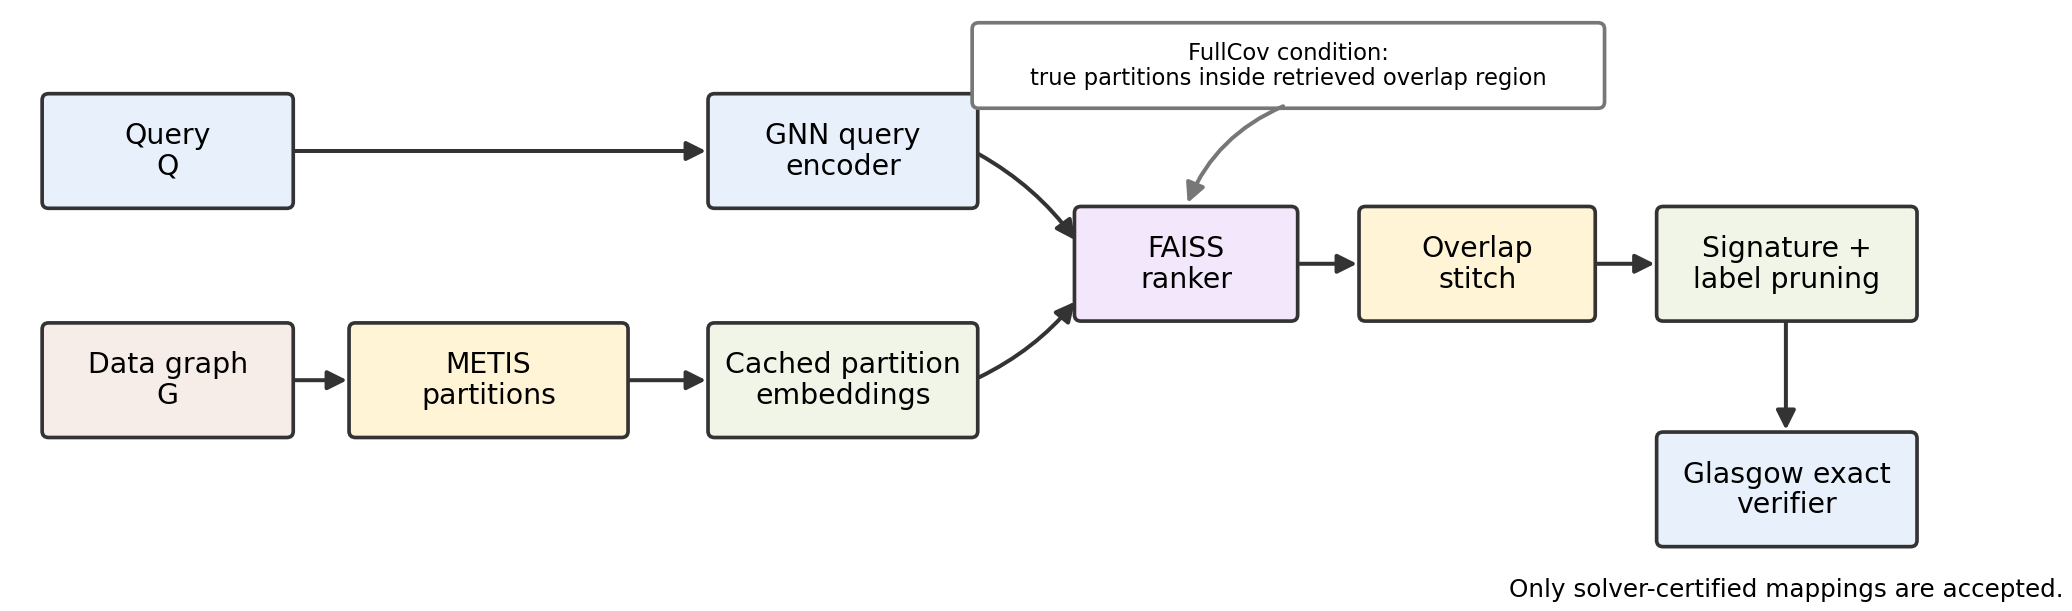
\includegraphics[width=\textwidth]{fig_jigsaw_pipeline.png}
\caption{\textbf{Jigsaw pipeline.} The learned component ranks partitions, but the only accepting step is Glasgow verification inside the stitched candidate graph. FullCov is the condition under which the candidate contains every partition needed by the planted match.}
\label{fig:pipeline}
\end{figure}

The data graph is partitioned into fine and coarse METIS blocks; coarse blocks are the retrieval units. For each query, Jigsaw computes an embedding $z_Q=f_\theta(Q)$ and ranks all coarse partitions by cosine similarity to cached partition embeddings, with FAISS providing fast top-$K$ retrieval (the encoder architecture is detailed in Appendix~\ref{app:encoder}). Hard partition boundaries are brittle: true query neighborhoods often cross coarse blocks, so Jigsaw stitches the retrieved partitions plus one-hop neighboring overlap, increasing recall before verification while still avoiding full-graph search. The stitched region is then filtered by typed structural signatures and exact labels; signatures match coarse type and feature fingerprints, and exact labels are especially important for negative-label queries. The final answer is produced only by the exact verifier.

\paragraph{FullCov objective.}
Standard contrastive training rewards high average similarity to positives, which can still leave one required partition ranked too low. Jigsaw optimizes the bottleneck. For each query $Q_i$, let $\mathcal{P}_i$ be its positive partitions and let $s_{ij}$ be the query-partition score. The objective combines multi-positive contrastive learning with a weak-positive term:
\begin{equation}
\mathcal{L}_{\mathrm{weak}}(i)=-\log
\frac{\exp(\min_{p\in\mathcal{P}_i}s_{ip}/\tau)}
{\exp(\min_{p\in\mathcal{P}_i}s_{ip}/\tau)+\sum_{n\in\mathcal{N}_i}\exp(s_{in}/\tau)}.
\end{equation}
Additional CVaR and barrier terms penalize positives that fall below the chosen retrieval budget. Partition embeddings are refreshed from cache, with live re-encoding of required positives so the weakest positive receives a usable gradient.

\paragraph{Why the weakest positive.}
The choice of $\min$ (and its CVaR relaxation) follows directly from the metric. $\mathrm{FullCov@K}(Q)=\mathbf{1}[\mathcal{T}(Q)\subseteq R_K(Q)]$ is a \emph{conjunction}: it succeeds only if \emph{every} $p\in\mathcal{P}_i$ is ranked within $K$, so failure is governed by the single worst-ranked required partition, $\min_{p\in\mathcal{P}_i} s_{ip}$, not the average positive score standard contrastive learning maximizes. Optimizing the average can raise mean recall while leaving one required partition below the budget -- exactly the failure exact verification cannot tolerate. CVaR (the mean of the worst $\alpha$-fraction of positives) is a smooth surrogate for the non-differentiable $\min$ that spreads gradient over the few hardest required partitions; this is why, in Table~\ref{tab:loss_ablation}, the objective improves fixed-budget FullCov most at the operating points the cascade uses, even though average recall barely moves. The retriever only proposes a candidate boundary; once $G_C$ is constructed, Glasgow gives exact answers, so a positive can fail two ways -- the boundary misses the planted solution, or the candidate grows too large and the solver times out -- and the benchmark records both.

\section{Experimental Protocol}

\paragraph{Datasets.}
We evaluate Cora~\cite{ref_cora}, OGBN-Arxiv~\cite{ref_ogb}, and the full heterogeneous OGBN-MAG. Cora is small enough for exact timing sanity checks; Arxiv is the main medium-scale benchmark; OGBN-MAG is a large heterogeneous graph (1{,}939{,}743 nodes across four node types joined by typed relations) and stresses the approach with both scale and relation-aware structure. It is modeled relation-aware (RGCN over retained node/edge types), not collapsed to an attribute-only homogeneous graph.

\paragraph{Label granularity.} The exact verifier matches on discrete vertex labels obtained by hashing each node's full attribute vector ($\sigma(v)=\mathrm{md5}(x_v)\bmod 10^{6}$), highly but not perfectly discriminative: the $10^{6}$ codebook admits collisions across the ${\sim}736$K featured MAG nodes, so a returned match is exact w.r.t.\ \emph{hashed-label} semantics rather than raw attribute equality (the one benchmark-level false positive per MAG method). These highly selective labels are the dominant reason every policy recovers all Cora and Arxiv positives once coverage is met: we call these \emph{label-rich} benchmarks and treat retrieval as a candidate-cost rather than accuracy lever. A coarser, more realistic labeling would weaken pruning and make retrieval more decisive -- a planted-benchmark limitation we discuss in Section~\ref{sec:limits}.

\paragraph{Queries and retrieval policies.}
The production matrix uses two query seeds, three target sizes (20/50/100), and 50 queries per type/size/seed. Positive families are single-partition, multi-fine, K-hop, degree K-hop, random walk, and multi-coarse; negatives are negative-label and negative-structure. All multi-region families use the corrected connected-positive generator. Six policies each isolate a failure mode: \textbf{Jigsaw} (learned GraphSAGE/RGCN partition ranker), \textbf{MeanFeat} (cosine on mean node features), \textbf{Mean-RRF} (reciprocal-rank fusion of the learned Jigsaw and MeanFeat rankings -- a configuration of our own retriever, not a nonparametric baseline), \textbf{TopoFeat} (coarse structural descriptors), \textbf{Random} (uninformed control), and \textbf{FilterAll} (all partitions to pruning/verification -- a recall ceiling, not a scalable retriever).

\paragraph{Partition and overlap scale.}
The partitions are deliberately balanced (MAG: 2{,}000 coarse partitions of median size 969, 10{,}000 fine partitions of median size 194). The overlap operator adds, for a selected partition, only the \emph{boundary nodes} of partitions sharing an edge with it -- a tight per-partition expansion ($5.4\times$ on MAG, not the loose $\approx$921K whole-neighbor-union bound). Breadth arises only when the cascade unions these overlaps across the retrieval budget; the verifier sees the much smaller pruned candidate of Table~\ref{tab:production_matrix}. Appendix~\ref{app:partitions} (Tables~\ref{tab:partition_sizes},~\ref{tab:partition_overlap}) gives the full scale, and Section~\ref{sec:shrinkage} dissects how much each cascade stage removes.

\paragraph{Metrics.}
We report FullCov@K and recall for retrieval ablations, and positive exact-solve rate, no-match accuracy, false positives, timeouts, candidate size, and wall-clock components for exact verification. Each dataset has exactly 288 production rows (6 methods, 2 seeds, 8 families, 3 sizes) of 50 logical queries each -- 14,400 method-query evaluations per dataset (43,200 across the three datasets) before budget expansion. Diagnostic variants are preserved separately without inflating the main grid.

\paragraph{Implementation and reproducibility.} Partitioning uses METIS; partition and query embeddings are indexed with FAISS; exact verification uses the Glasgow Subgraph Solver, invoked on the pruned candidate graph exported in \texttt{vertexlabelledlad} format with node features discretized to integer vertex labels. All reported timings are per-query wall-clock on Google Cloud \texttt{CPU\_X\_8} instances (8 vCPUs), with the exact verifier run under a bounded per-query time budget (30\,s). Encoders are six residual message-passing blocks ($\mathtt{SAGEConv}$ for Cora/Arxiv, $\mathtt{RGCNConv}$ for MAG) producing $L_2$-normalized 128-dimensional embeddings. Trained encoders, query seeds, partition hierarchies, and the hash-manifested benchmark bundle will be released to support full reproduction.

\section{Results}

\subsection{FullCov Training Improves Retrieval}

Table~\ref{tab:loss_ablation} (visualized in Figure~\ref{fig:fullcov_ablation}) gives the matched-budget Arxiv retrieval result. All rows use the same locked K-hop query seeds and 9,000 optimizer steps. The FullCov objective improves the fixed-budget operating points most relevant to bounded exact verification.

\begin{table}[t]
\centering
\caption{\textbf{Matched Arxiv retrieval objective ablation.} Fixed retrieval budgets, two locked query seeds, two training replicates for control/final.}
\label{tab:loss_ablation}
\small
\setlength{\tabcolsep}{5pt}
\begin{tabular}{lcccc}
\toprule
\textbf{Objective} & \textbf{FullCov@20} & \textbf{FullCov@50} & \textbf{FullCov@100} & \textbf{Mean worst rank} \\
\midrule
Contrastive control & 21.7\% & 39.0\% & 66.0\% & 74.02 \\
FullCov objective & \textbf{26.0\%} & \textbf{48.8\%} & \textbf{82.0\%} & \textbf{58.97} \\
\midrule
McNemar $p$ & $4.6{\times}10^{-3}$ & $9.8{\times}10^{-6}$ & $4.0{\times}10^{-10}$ & -- \\
\bottomrule
\end{tabular}
\end{table}

The effect is not a change in feasibility: the locked K-hop suite has zero queries impossible at $K=20,50,100$; average true coarse footprint is 6.37 and maximum footprint is 17. Misses are ranking errors, which the objective reduces by explicitly optimizing the weakest required partition. This is the cleanest evidence for the training objective: it uses the same query seeds and training budget for both models, so the improvement is not explained by easier queries or longer optimization. The largest gain appears at FullCov@100, where the downstream verifier has enough room to benefit from better ordering but still cannot search the whole graph -- the operating point the cascade actually uses.

\subsection{Three-Dataset Production Matrix}

Table~\ref{tab:production_matrix} reports the cleaned production metrics. Positive queries measure exact planted-match recovery; negative queries measure correct no-match behavior. The table also includes false positives, solver timeouts, average candidate nodes, end-to-end runtime, and verifier time. Headline table values are traced in \texttt{HEADLINE\_NUMBERS.csv} and \texttt{CANONICAL\_SOURCES.md}; legacy normalized summaries are retained only for provenance and encoder-independent rows.

\begin{table}[t]
\centering
\caption{\textbf{Final production metrics across Cora, OGBN-Arxiv, and OGBN-MAG.} Pos. is planted positive exact-solve rate. Neg. is correct no-match rate. FP is false positives on negatives; TO is solver timeouts. \textbf{Pos.\ is at the matched half-partition budget} $K{=}10/100/1000$ (Cora/Arxiv/MAG); a matched \emph{fraction} is used because $K$ is absolute and partition totals differ (20/200/2{,}000). At this budget policies separate (random/topology $31$--$51\%$: $31$--$38\%$ Cora/Arxiv, $37$--$51\%$ MAG). $^\ddagger$\,FilterAll is budget-independent (all partitions) = the exhaustive ceiling; Cora/Arxiv reach $100\%$ only there, not as a retrieval result. Neg.\ is no-match rate; candidate nodes/runtimes are per-query averages (verifier input medians $51/50$ on Cora/Arxiv); full solved-by-$K$ curves in Appendix~\ref{app:family}. The MAG Jigsaw/Mean-RRF rows use the deployed walk-aware encoder; the rest are encoder-independent. $^\S$\,FeatureIndex is the classical GraphGrep/gIndex-style label-coverage index; under these near-unique labels it is the strongest bounded retriever, exceeding the learned model (positives only; no-match/FP omitted). For the two MAG walk-aware rows the Neg.\,/\,FP\,/\,TO columns are carried from the generic-encoder benchmark, and for the Cora/Arxiv learned rows the candidate-size and runtime columns are from the earlier full-budget run.}
\label{tab:production_matrix}
\scriptsize
\setlength{\tabcolsep}{2.5pt}
\begin{tabular}{llrrrrrrr}
\toprule
\textbf{Dataset} & \textbf{Method} & \textbf{Pos. \%} & \textbf{Neg. \%} & \textbf{FP} & \textbf{TO} & \textbf{Cand. nodes} & \textbf{Total s} & \textbf{Solver ms} \\
\midrule
Cora & Jigsaw & 94.2 & 100.0 & 0 & 0 & 2.5K & 0.09 & 7.9 \\
Cora & Mean-RRF & 93.8 & 100.0 & 0 & 0 & 2.4K & 0.09 & 8.3 \\
Cora & MeanFeat & 88.8 & 100.0 & 0 & 0 & 3.5K & 0.11 & 7.4 \\
Cora & TopoFeat & 33.4 & 100.0 & 0 & 0 & 9.5K & 0.22 & 3.2 \\
Cora & Random & 31.3 & 100.0 & 0 & 0 & 9.6K & 0.21 & 3.2 \\
Cora & FilterAll$^\ddagger$ & 100.0 & 100.0 & 0 & 0 & 0.8K & 0.07 & 11.3 \\
\midrule
Arxiv & Jigsaw & 92.8 & 100.0 & 0 & 0 & 0.2K & 0.59 & 12.9 \\
Arxiv & Mean-RRF & 94.0 & 100.0 & 0 & 0 & 0.2K & 0.41 & 16.0 \\
Arxiv & MeanFeat & 88.9 & 100.0 & 0 & 0 & 0.2K & 0.39 & 16.5 \\
Arxiv & TopoFeat & 33.2 & 100.0 & 0 & 0 & 0.3K & 0.75 & 5.1 \\
Arxiv & Random & 37.7 & 100.0 & 0 & 0 & 0.3K & 0.77 & 5.4 \\
Arxiv & FilterAll$^\ddagger$ & 100.0 & 100.0 & 0 & 0 & 0.1K & 0.35 & 16.9 \\
\midrule
MAG & Jigsaw & \textbf{88.6} & 99.8 & 1 & 23 & 138.1K & 6.97 & 81.9 \\
MAG & Mean-RRF & 85.4 & 99.7 & 1 & 16 & 137.1K & 5.38 & 67.9 \\
MAG & FeatureIndex$^\S$ & \textbf{96.7} & -- & -- & 24 & 59.4K & 2.39 & 118.8 \\
MAG & MeanFeat & 64.6 & 99.8 & 1 & 10 & 212.1K & 8.02 & 27.5 \\
MAG & TopoFeat & 37.1 & 99.8 & 1 & 1 & 235.6K & 8.07 & 5.2 \\
MAG & Random & 51.4 & 99.8 & 1 & 8 & 282.1K & 9.54 & 19.9 \\
MAG & FilterAll$^\ddagger$ & 98.4 & 99.8 & 1 & 30 & 443.8K & 5.85 & 288.6 \\
\bottomrule
\end{tabular}
\end{table}

Cora and Arxiv reach $100\%$ only at the exhaustive all-partition budget (their 20/200 partitions), so that figure is the FilterAll-equivalent ceiling, not a retrieval result. At the cross-dataset-comparable half-partition budget the overlap-aware GraphSAGE retriever solves Cora $94.2\%$ and Arxiv $92.8\%$, with random/topology collapsing to $31$--$38\%$ (Cora/Arxiv; $37$--$51\%$ on MAG). Crucially, the overlap-aware retrain is what closes the Arxiv gap: a retriever trained without overlap supervision reached only $74.1\%$ at this budget, versus $92.8\%$ here (Cora was already near-saturated, $95.4\%\!\to\!94.2\%$). The learned retriever is competitive but not uniquely best (Mean-RRF $93.8\%$/$94.0\%$), and on MAG a classical label index is in fact the strongest bounded retriever ($96.7\%$, below), so we frame the retriever as replaceable. MAG is the stress case: random and topology degrade sharply, mean features help, and the deployed walk-aware model reaches \textbf{88.6\%} while sending the verifier $3.2\times$ fewer candidate nodes than FilterAll (138K vs.\ 444K). FilterAll is higher at 98.4\%, but it gives the verifier all partitions and is a recall ceiling rather than a scalable policy. \textbf{The cascade also never holds the whole graph resident:} it admits partitions one at a time and prunes on node-ID and label sets before materializing edges, so a conservative streaming serve (resident cache of eight partitions, survivor edges fetched in a second pass) peaks at \textbf{2.4\,GB} across a 54-query MAG grid (all six families) versus \textbf{10.2\,GB} to hold MAG for a direct solve -- a $4.2\times$ reduction -- recovering $46/54$ planted matches (all easy-family queries; the 8 misses are random-walk/multi-coarse) and solving components of median $110$ nodes (max $9{,}497$) in $5$\,ms--$8.4$\,s.

\paragraph{Label-selectivity crossover.} The benchmark's near-unique md5 labels flatter exact-label methods: a classical label-coverage index (\textbf{FeatureIndex}, GraphGrep/gIndex-style) is in fact the strongest bounded retriever here ($96.7\%$ solve, median worst-true-partition rank $104$ of $2{,}000$), ahead of the learned GNN ($88.6\%$; median rank ${\sim}900$). This is a property of the labels, not the framework: rerunning the MAG matrix at coarse $39$-class labels \emph{inverts} the ranking result---the learned retriever has better worst-true-partition ranks in each query family, while the complete coarse-label solve runs are statistically tied (FeatureIndex $63.4\%$; learned GNN variants $63$--$64\%$). The crossover is strongest on the model-independent ranking metric (partition ranking uses the label-agnostic embedding); end-to-end solve is corroborating only, with candidate size, timeouts, and false positives genuinely label-dependent. The finding: learned retrieval helps precisely as labels stop being selective, but the current evidence is a localization win, not a solve-rate win. The same experiment exposes the learned retriever's real weakness---it localizes contained queries near-perfectly (single/multi-fine rank $3$--$7$) but is near-random on spatially-extended families (k-hop, degree-k-hop, random-walk; rank ${\approx}1700$ of $2{,}000$), because the embedding does not discriminate all $16$--$30$ partitions they span. A battery of inference-time remedies (subquery MaxSim, finer partitions, fine- and coarse-level overlap, dual-granularity late interaction) leaves FullCov@1000 within ${\approx}2$ points on these families, so the issue is representation, not aggregation (Appendix~\ref{app:probes}); the crossover itself generalizes to Cora and Arxiv, where the winner flips with an offline label-selectivity statistic, so Jigsaw selects its retriever by label regime. Jigsaw is therefore \emph{retriever-agnostic}---its contribution is memory-bounded exact verification, not a superior neural retriever.

The MAG result has a clear lower bound: \emph{direct exact matching on the full graph with no retrieval} solves \textbf{0 of 15} sampled K-hop queries, every one exhausting the time budget, so retrieval is a prerequisite, not an optimization. The crossover is not unique to MAG: across scales (Table~\ref{tab:scaling_latency}, Figure~\ref{fig:scaling}) the identical direct solver clears all 15 Cora queries but already collapses to \textbf{0 of 15} on OGBN-Arxiv (169K nodes), while the Jigsaw cascade stays feasible by handing the verifier a $\sim\!50$-node pruned candidate -- placing the tractability crossover between Cora and Arxiv, well below the largest graph. The point is not that one retriever is uniquely good -- Mean-RRF (85.4\%) is not a competitor but a second \emph{configuration of Jigsaw's own retriever} (learned ranking fused with the mean-feature ranking), and the pure learned ranker leads it by $3.2$ points; both dominate the genuinely unlearned mean-feature baseline ($64.6\%$, a $+24$ gap) -- but that \emph{all} of these turn an infeasible problem into a tractable one along a recall-vs-cost frontier (full numbers in Appendix~\ref{app:mag_narrative}).

\begin{figure}[tb]
\centering
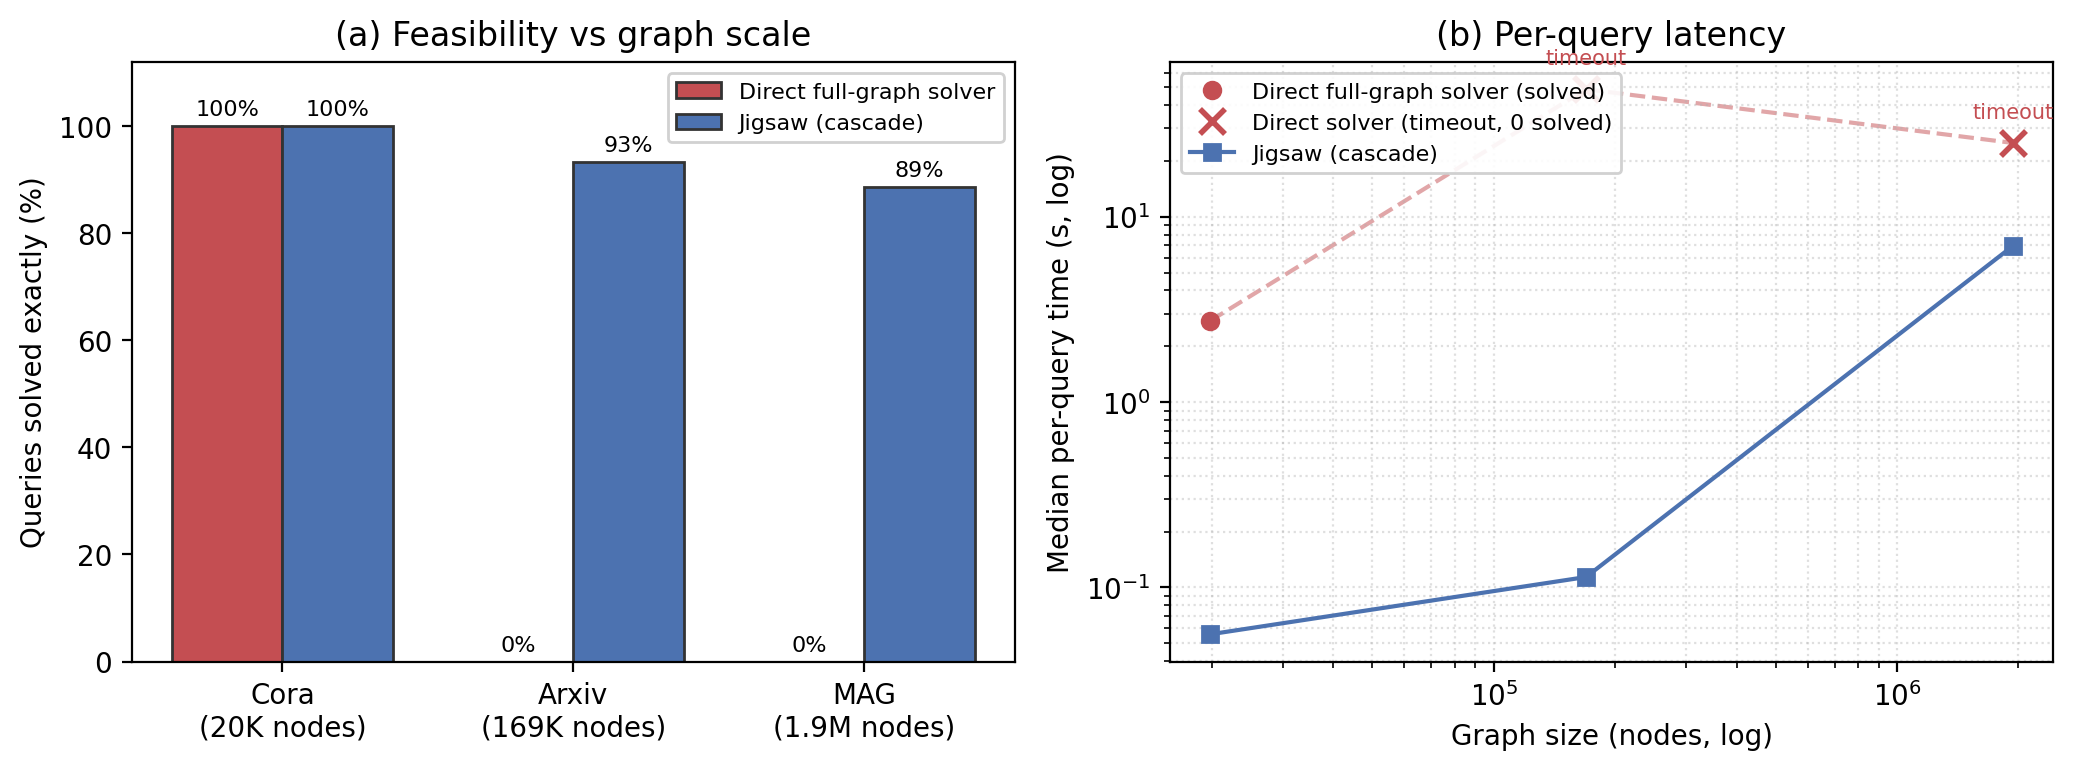
\includegraphics[width=0.82\textwidth]{fig_scaling_feasibility.png}
\caption{\textbf{Jigsaw makes the exact solver's domain tractable.} (a) Feasibility vs.\ graph scale: the direct full-graph solver clears all Cora queries but solves \emph{none} at Arxiv (169K) or MAG (1.9M) scale, while the Jigsaw cascade stays feasible throughout (100/93/89\%). (b) Per-query latency (log--log): the direct solver is censored at its time budget (X = timeout, 0 solved) for Arxiv and MAG; Jigsaw runs one-to-three orders of magnitude faster because the verifier sees only the retrieved-and-pruned candidate. Matched K-hop queries; numbers in Table~\ref{tab:scaling_latency}.}
\label{fig:scaling}
\end{figure}

\begin{table}[t]
\centering
\caption{\textbf{Scaling and latency: direct full-graph solver vs.\ Jigsaw cascade}, on matched K-hop queries (seed 20260607, target sizes 20/50/100, 5 each = 15 queries per dataset; MAG cascade is the production-matrix neural retriever over its eight query families). The direct solver hands Glasgow the entire graph; Jigsaw hands it the retrieved, overlapped, and pruned candidate. ``Median time'' is wall-clock per query (retrieval${+}$candidate${+}$solve for Jigsaw; solve for the direct baseline). $^\dagger$ The direct solver is given the same 30\,s solve budget as the verifier; reported times are wall-clock to abort, which exceeds the request because Glasgow does not preempt cleanly (${\approx}49$\,s on Arxiv; the MAG ${\approx}25$\,s is dominated by loading the 1.9M-node target before abort). The run is aborted with no match returned. $^\ast$ The MAG cascade cell is the per-query \emph{mean} total from the production matrix (Table~\ref{tab:production_matrix}); the Cora/Arxiv cascade cells are true medians.}
\label{tab:scaling_latency}
\small
\begin{tabular}{l r c r c r r}
\toprule
 & & \multicolumn{2}{c}{Direct full-graph solver} & \multicolumn{2}{c}{Jigsaw cascade} & Cand.\ \\
\cmidrule(lr){3-4}\cmidrule(lr){5-6}
Dataset & Nodes & Solved & Med.\ time & Solved & Med.\ time & nodes \\
\midrule
Cora  & 19.8K & 15/15 & $2.74$\,s & 15/15 & $\mathbf{0.06}$\,s & 51 \\
Arxiv & 169K  & \textbf{0/15}$^\dagger$ & ${\approx}49$\,s & 14/15 & $\mathbf{0.11}$\,s & 50 \\
MAG   & 1.9M  & \textbf{0/15}$^\dagger$ & ${\approx}25$\,s & 88.6\% & $6.97$\,s$^\ast$ & -- \\
\bottomrule
\end{tabular}
\end{table}

Bootstrap 95\% confidence intervals and paired exact-McNemar tests on the MAG solve rate confirm this ordering among the interchangeable retrieval \emph{components} (full statistics, per-family solve rates, and budget curves in Appendices~\ref{app:mag_narrative} and~\ref{app:family}). These are comparisons among retrieval components; the contribution is the surrounding system -- exact matching at scale without holding the graph resident, with FullCov securing coverage on the hard families.

\subsection{Candidate-Shrinkage Cascade and Selective Overlap}
\label{sec:shrinkage}

A natural objection is that if one-hop overlap is broad, the partition boundary may not be doing real work. We test this by measuring the per-query cascade $\text{full graph} \to \text{overlap} \to \text{signature} \to \text{label-pruned} \to \text{solver}$ on 14{,}400 MAG queries (10{,}800 positives) from the generic-mix-encoder run at the decided budget. Three facts emerge. \textbf{(1) Overlap is broad, but partition ranking still removes most of the graph:} the median overlap union is 59\% of MAG for Jigsaw (vs.\ 73--83\% for mean-feature, random, and topology retrieval), yet after identical pruning Jigsaw's candidate is a median 84.5K nodes versus 544K for FilterAll (medians; the production matrix reports means, 138.1K vs 443.8K) -- a $6.4\times$ reduction attributable to ranking alone.

\textbf{(2) All recall loss occurs at the overlap stage; pruning is coverage-lossless.} This is not merely empirical but a property of the pruning operator.

\begin{proposition}[Lossless pruning]
\label{prop:lossless}
Let the pruning token $\sigma(\cdot)$ be a node attribute that the matching semantics preserve, i.e.\ any valid embedding $\phi$ of $Q$ into $G$ satisfies $\sigma(\phi(q))=\sigma(q)$ for every query node $q$ (vertex-labelled matching, with $\sigma$ derived from node type and feature labels). Prune the candidate $G_C$ to $G_C'=\{v\in G_C : \sigma(v)\in \sigma(V_Q)\}$. Then for any embedding $\phi$ with $\phi(V_Q)\subseteq G_C$, we have $\phi(V_Q)\subseteq G_C'$. Hence pruning preserves node coverage: $\mathrm{FullCov}$ is unchanged.
\end{proposition}
\noindent\emph{Proof.} For $q\in V_Q$, $\sigma(\phi(q))=\sigma(q)\in\sigma(V_Q)$, so $\phi(q)$ satisfies the keep condition and is retained. Thus every matched node survives. $\square$

The cascade signatures (node type $\times$ feature-bit hashes) and the exact label filter are such attribute invariants, so Proposition~\ref{prop:lossless} applies; a \emph{degree}-based token would not be matching-invariant ($\deg(\phi(q))\ge\deg(q)$ only), which is why the pipeline prunes on attributes, not degree. Empirically, for every policy the planted-match survival rate after overlap equals that after pruning (Jigsaw $87\%$ both, in this generic-encoder diagnostic whose end-to-end solve is $86.0\%$), so the solve ceiling is set entirely by whether the retrieved-plus-overlapped region \emph{contains} the match.

\textbf{(3) Latency is dominated by candidate construction, not solving} (per-query build $\gg$ solve; Appendix~\ref{app:mag_narrative}): the verifier is cheap, and assembling the broad overlap union is the cost.

\paragraph{Why broad overlap is mostly wasted, and the selective-overlap fix.}
The breadth of one-hop overlap is not buying recall. A controlled probe over the cached MAG index shows that when retrieval misses a true partition, one-hop overlap recovers it for 94\% of K-hop queries but only 62\% of random-walk queries, because overlap reaches only the \emph{boundary} nodes of retrieved partitions, never the interior of a fully unselected one. Broad overlap thus inflates candidate size when retrieval already succeeded, without repairing the misses. This motivates \emph{selective overlap}: expand each selected partition only to its highest-support neighbors (ranked by bridge boundary count) and/or to label-compatible nodes. Trimming only overlap nodes and never partition interiors preserves the recall partition selection provides while shrinking the dominant build cost: in the probe (pooled over the four query families), capping each partition to its eight strongest neighbors cuts the overlap union by ${\approx}3.1\times$, label-compatible expansion by ${\approx}5.0\times$, and the two combined by over $6\times$, at no cost in candidate \emph{size} (a recall-preserving claim needs the aligned-hierarchy re-run we leave to future work). We provide these as configurable operators (\texttt{--overlap-max-parts}, \texttt{--overlap-min-support}, \texttt{--overlap-label-compatible}) and identify selective overlap as the principal systems lever for closing the FilterAll gap at lower latency, since candidate construction is volume-bound (Appendix~\ref{app:mag_narrative}).

\subsection{Negative Queries and Soundness}

Jigsaw never accepts a match from the neural model alone -- the only accepting step is Glasgow verification -- so negative-label and negative-structure queries test the no-match behavior of candidate construction and the verifier. Audited no-match accuracy is 100.0\% for Cora and Arxiv and 99.7--99.8\% for selected MAG rows, with at most one false positive per method. These are not verifier hallucinations: a returned Glasgow mapping is a real isomorphism inside the candidate, so when the generator perturbs a query but the data graph happens to contain another matching structure, the solver is correct and the failure is benchmark-level. A stronger negative benchmark would certify non-existence globally -- precisely the expensive exact problem that motivates retrieval-constrained verification.

\section{Discussion and Limitations}
\label{sec:limits}

Jigsaw should be read as an exact-verification system with a learned boundary, not a proof of global completeness: if retrieval misses a necessary region the solver cannot recover the planted match, and FullCov makes that failure mode measurable. It is strongest for static attributed graphs with repeated query workloads, where partitioning, embedding, and FAISS indexing amortize. Cora and Arxiv show no large neural advantage because labels and pruning dominate once coverage is sufficient; MAG is where policies separate. FeatureIndex is strongest under near-unique labels, while learned retrieval becomes the better localizer as labels coarsen; FilterAll is an exhaustive upper bound, not a scalable retriever.

The main empirical limitation is comparison scope. We compare against classical feature- and structure-index rankers (the MeanFeat/TopoFeat policies, GraphGrep/gIndex-style filters), a no-retrieval exact control (full-graph Glasgow, $0/15$ MAG queries), an exhaustive FilterAll upper bound, and uninformed feature/random/topology retrievers, but not learned node-alignment matchers (NeuroMatch, GLSearch): trained on small graphs (hundreds of nodes) with the query \emph{contained} in one target, they have no scalable route to million-node graphs or cross-partition queries, so they are a different problem class rather than an omitted baseline. We benchmark scalable filter-and-verify matchers (CFL-Match, DP-iso, GQL): they solve Cora/Arxiv and MAG once loaded, so our infeasibility claim is scoped to the CP-based Glasgow solver (0/15 on MAG) and to the memory and low-selectivity regimes where they degrade (12/27 at coarse labels). The residence axis has out-of-core and distributed precedents (DUALSIM~\cite{ref_dualsim}, STwig/Trinity~\cite{ref_trinity}, G-thinker~\cite{ref_gthinker}); Jigsaw differs in bounding residence by learned region relevance on one machine, makes no claim of outperforming them, and its memory benefit must be weighed against one-time offline cost (partitioning, encoder training, embedding the partition bank), so it is strongest for graphs that cannot be held resident or for multi-tenant/cold-start serving rather than a single amortizable load. A scoped GNN-PE public-release diagnostic is reported below. Two further limitations: the negative families are audited synthetic no-match tests, not a global proof of non-existence; and queries are planted connected subgraphs on static single graphs, not an external pattern workload. On these label-rich planted benchmarks several policies localize the candidate well once coverage is met, so we do not claim the learned retriever dominates cheaper ones on \emph{recall}; its role is to make the candidate small and memory-bounded, and FullCov is what secures coverage on the hard families where cheaper policies fail. Establishing a regime where a learned retriever is also decisive on recall would need harder, weakly-labeled or non-planted workloads.

\paragraph{GNN-PE public-release diagnostic.}
Beyond the internal retrieval policies, our external baselines are the direct-solver control (Table~\ref{tab:scaling_latency}, $0/15$ on Arxiv/MAG) and this GNN-PE diagnostic. We ran the released GNN-PE pipeline on Cora: its bundled self-test passes, but after class-label export, build/serialization repairs, and an $e=128$ stress test it recovered only $7/24$ planted positives at $e=4$ and $5/24$ at $e=128$ ($0/6$ at size 100) -- a higher embedding dimension did not help. The released executable builds embeddings and indexes directly and exposes no separate supervised training step for these runs, so this is public-release feasibility, not a full-recipe reproduction; the pipeline remains unusable for our planted-query protocol without deeper upstream changes.

\section{Conclusion}

Jigsaw connects learned graph retrieval and exact subgraph verification through a measurable coverage condition: FullCov raises the probability that all required regions are retrieved, while overlap and pruning make exact verification tractable. Jigsaw is \emph{retriever-agnostic}: it selects bounded retrievers by offline label selectivity (Appendix~\ref{app:probes}). The contribution is exact verification made usable on large static graphs under bounded memory.

% ============================ APPENDIX ============================

\begin{thebibliography}{25}

\bibitem[McCreesh et al.(2020)]{ref_glasgow}
McCreesh, C., Prosser, P., Trimble, J.: The Glasgow Subgraph Solver: Using Constraint Programming to Tackle Hard Subgraph Isomorphism Problem Variants. In: CP 2020, LNCS, vol. 12333, pp. 316--333. Springer (2020)

\bibitem[Xu et al.(2019)]{ref_gin}
Xu, K., Hu, W., Leskovec, J., Jegelka, S.: How Powerful are Graph Neural Networks? In: ICLR (2019)

\bibitem[Cordella et al.(2004)]{ref_vf2}
Cordella, L.P., Foggia, P., Sansone, C., Vento, M.: A (Sub)Graph Isomorphism Algorithm for Matching Large Graphs. IEEE TPAMI \textbf{26}(10), 1367--1372 (2004)

\bibitem[Johnson et al.(2021)]{ref_faiss}
Johnson, J., Douze, M., J\'egou, H.: Billion-Scale Similarity Search with GPUs. IEEE Trans. Big Data \textbf{7}(2), 535--547 (2021)

\bibitem[Karypis and Kumar(1998)]{ref_metis}
Karypis, G., Kumar, V.: A Fast and High Quality Multilevel Scheme for Partitioning Irregular Graphs. SIAM J. Sci. Comput. \textbf{20}(1), 359--392 (1998)

\bibitem[Hu et al.(2020)]{ref_ogb}
Hu, W., et al.: Open Graph Benchmark: Datasets for Machine Learning on Graphs. In: NeurIPS (2020)

\bibitem[Garey and Johnson(1979)]{ref_garey}
Garey, M.R., Johnson, D.S.: Computers and Intractability: A Guide to the Theory of NP-Completeness. W.H. Freeman (1979)

\bibitem[Bonnici et al.(2013)]{ref_ri}
Bonnici, V., Giugno, R., Pulvirenti, A., Shasha, D., Ferro, A.: A Subgraph Isomorphism Algorithm and Its Application to Biochemical Data. BMC Bioinformatics \textbf{14}(Suppl 7), S13 (2013)

\bibitem[Solnon(2010)]{ref_lad}
Solnon, C.: AllDifferent-Based Filtering for Subgraph Isomorphism. Artificial Intelligence \textbf{174}(12--13), 850--864 (2010)

\bibitem[Sen et al.(2008)]{ref_cora}
Sen, P., Namata, G., Bilgic, M., Getoor, L., Galligher, B., Eliassi-Rad, T.: Collective Classification in Network Data. AI Magazine \textbf{29}(3), 93--106 (2008)

\bibitem[Ying et al.(2020)]{ref_neuromatch}
Ying, R., et al.: Neural Subgraph Matching. arXiv:2007.03092 (2020)

\bibitem[Ye et al.(2024)]{ref_gnnpe}
Ye, Y., Lian, X., Chen, M.: Efficient Exact Subgraph Matching via GNN-based Path Dominance Embedding. Proc. VLDB Endow. \textbf{17}(7), 1628--1641 (2024)

\bibitem[Liu et al.(2021)]{ref_glsearch}
Liu, Y., et al.: GLSearch: Maximum Common Subgraph Detection via Learning to Search. In: ICML (2021)

\bibitem[Liu et al.(2020)]{ref_nsic}
Liu, X., Pan, H., He, M., Song, Y., Jiang, X., Shang, L.: Neural Subgraph Isomorphism Counting. In: KDD (2020)

\bibitem[Han et al.(2013)]{ref_turboiso}
Han, W.S., Lee, J., Lee, J.H.: TurboISO: Towards Ultrafast and Robust Subgraph Isomorphism Search in Large Graph Databases. In: SIGMOD, pp. 337--348 (2013)

\bibitem[Bi et al.(2016)]{ref_cflmatch}
Bi, F., Chang, L., Lin, X., Qin, L., Zhang, W.: Efficient Subgraph Matching by Postponing Cartesian Products. In: SIGMOD, pp. 1199--1214 (2016)

\bibitem[Han et al.(2019)]{ref_daf}
Han, M., Kim, H., Gu, G., Park, K., Han, W.S.: Efficient Subgraph Matching: Harmonizing Dynamic Programming, Adaptive Matching Order, and Failing Set Together. In: SIGMOD, pp. 1429--1446 (2019)

\bibitem[Carletti et al.(2018)]{ref_vf3}
Carletti, V., Foggia, P., Saggese, A., Vento, M.: Challenging the Time Complexity of Exact Subgraph Isomorphism for Huge and Dense Graphs with VF3. IEEE Trans. Pattern Anal. Mach. Intell. \textbf{40}(4), 804--818 (2018)

\bibitem[Zeng et al.(2020)]{ref_gsi}
Zeng, L., Zou, L., \"Ozsu, M.T., Hu, L., Zhang, F.: GSI: GPU-friendly Subgraph Isomorphism. In: ICDE, pp. 1249--1260 (2020)

\bibitem[Sun and Luo(2020)]{ref_survey}
Sun, S., Luo, Q.: In-Memory Subgraph Matching: An In-depth Study. In: SIGMOD, pp. 1083--1098 (2020)

\bibitem[Kim et al.(2016)]{ref_dualsim}
Kim, H., Lee, J., Bhowmick, S.S., Han, W.-S., Lee, J., Ko, S., Jarrah, M.H.A.: DUALSIM: Parallel Subgraph Enumeration in a Massive Graph on a Single Machine. In: SIGMOD, pp. 1231--1245 (2016)

\bibitem[Sun et al.(2012)]{ref_trinity}
Sun, Z., Wang, H., Wang, H., Shao, B., Li, J.: Efficient Subgraph Matching on Billion Node Graphs. Proc. VLDB Endow. \textbf{5}(9), 788--799 (2012)

\bibitem[Yan et al.(2020)]{ref_gthinker}
Yan, D., Guo, G., Chowdhury, M.M.R., \"Ozsu, M.T., Ku, W.-S., Lui, J.C.S.: G-thinker: A Distributed Framework for Finding Qualified Subgraphs in a Big Graph with Load Balancing. In: ICDE (2020)

\end{thebibliography}

\appendix

\section{Expanded MAG Results and Statistical Significance}
\label{app:mag_narrative}

This appendix expands the condensed MAG discussion in Appendix~\ref{app:family} and the production matrix (Table~\ref{tab:production_matrix}); no number differs from the body; the detail is relocated here only to keep the body within the page limit.

\paragraph{Candidate cost on Cora and Arxiv.} With the overlap-aware GraphSAGE retrievers, the verifier input stays small: a median of $51$ pruned candidate nodes on Cora and $50$ on Arxiv (means $\sim\!0.9$K and $88$), far below random/topology retrieval. At the half-partition budget these retrievers solve $94.2\%$ (Cora) and $92.8\%$ (Arxiv); the $100\%$ reached only at the all-partition budget is the exhaustive ceiling. Labels, component decomposition, and exact pruning keep the verifier input tiny once the planted region is inside the candidate, so the retriever's measurable effect on these graphs is candidate-domain cost.

\paragraph{The MAG lower bound and scaling crossover, in full.} The MAG result is the most important systems result in the paper: the problem is not merely solved by labels, and the method should be judged against both cheap baselines and an exhaustive upper bound. \emph{Direct exact matching on the full graph with no retrieval} (the query handed to Glasgow against the entire 1.9M-node MAG target) solves \textbf{0 of 15} sampled K-hop queries, every one exhausting the time budget (median ${\approx}25$\,s per query including target loading). The direct Glasgow solve is therefore infeasible at this scale -- retrieval is a prerequisite for the CP solver, not an optimization (filter-and-verify matchers solve MAG once the whole graph is loaded but require full residence, Section~\ref{sec:limits}). Running the identical direct solver on matched K-hop queries across scales (Table~\ref{tab:scaling_latency}), it solves all 15 Cora queries (19.8K nodes) in a median $2.74$\,s, but already collapses to \textbf{0 of 15} on OGBN-Arxiv (169K nodes), every query exhausting the budget at ${\approx}49$\,s. The same Jigsaw cascade solves those instances exactly in a median $0.06$\,s on Cora and $0.11$\,s on Arxiv (14/15) -- a ${\approx}49\times$ speedup where the solver is feasible and an infeasible-to-feasible jump where it is not -- by handing the verifier a pruned candidate of $\sim\!50$ nodes instead of the full $169$K. The retriever is a component on a recall-vs-cost frontier: FeatureIndex is strongest under near-unique MAG labels, FilterAll is the recall ceiling at the highest verifier cost, and the learned retriever is a useful memory-bounded operating point, especially once labels coarsen. Jigsaw uses fewer MAG candidate nodes than FilterAll (138K versus 444K) and far lower verifier time (82 ms versus 289 ms), although candidate construction remains the dominant cost.

\paragraph{Statistical significance.}
Bootstrap 95\% confidence intervals on the MAG positive solve rate (n${=}1800$ queries per method) and paired exact-McNemar tests (pairing per query so wins/losses count only queries two policies decide differently) confirm the ordering. Among the retrieval \emph{components}, the FullCov-trained retriever significantly outperforms the other learned and feature retrievers (Mean-RRF, re-evaluated under the same walk-aware encoder, 92 vs 35 wins, $p{=}4.4{\times}10^{-7}$; mean features / random / topology $p<10^{-76}$), and FilterAll significantly exceeds it (225 vs 2 wins, $p{=}2.4{\times}10^{-64}$) as the exhaustive ceiling; the latter four are encoder-independent and reported against the base-encoder Jigsaw. These are comparisons \emph{among retrieval components}; the paper's contribution is the surrounding system -- exact matching at million-node scale without holding the graph resident. The retriever keeps the candidate both small and memory-bounded, sending the verifier $3.2\times$ fewer candidate nodes than the exhaustive FilterAll ceiling, and FullCov secures coverage on the hard families where cheaper policies fail.

\paragraph{Candidate construction is volume-bound.} Latency is dominated by candidate construction, not solving: mean per-query candidate-build time is 3.4\,s (Jigsaw) and 5.5\,s (FilterAll), against 0.25\,s of exact solving (Section~\ref{sec:shrinkage}, fact 3). These build and solve means are measured on the generic-encoder shrinkage diagnostic; the production-matrix per-query totals of Table~\ref{tab:production_matrix} additionally include retrieval time and use the walk-aware encoder, so they are not the arithmetic sum of this build and solve. The dominant build cost is set by the number of admitted nodes, not the union algorithm: replacing the set-union with a vectorized tensor union is verified identical but only $0.5$--$0.9\times$ as fast, so the build cost falls only when the number of admitted nodes falls. This is why selective overlap, which reduces node volume, is the principal latency lever.

\section{Retrieval Remedies and Cross-Dataset Selectivity}
\label{app:probes}

\paragraph{The label-selectivity crossover generalizes.} Repeating the retrieval comparison on Cora and OGBN-Arxiv (retrieval-only, identical query families, $n{=}540$ each) reproduces the MAG inversion (Table~\ref{tab:selectivity_xd_log}). It tracks an offline statistic---the median number of partitions a label spans (Cora feature labels $1$, class $12$; Arxiv feature $1$, class $124.5$). Under near-unique feature labels the classical index ties the learned retriever on contained families and wins overall (Cora rank $2$ vs.\ $5$; Arxiv $4$ vs.\ $44$); under realistic class labels it collapses toward random (Arxiv $104$ of $200$) while the learned retriever wins every family (Cora $5$ vs.\ $7$; Arxiv $44$ vs.\ $104$; per-query sign test $p<10^{-30}$ in both regimes, $n{=}540$). Selecting the retriever by this offline signal is a deployable, non-oracle portfolio; on Cora/Arxiv it is a localization (retrieval-rank) result, corroborated end-to-end only on MAG.

\begin{table}[h]
\centering
\caption{Cross-dataset label-selectivity crossover: overall median worst-true-partition rank (lower is better; retrieval-only, $n{=}540$).}
\label{tab:selectivity_xd_log}
\small
\begin{tabular}{lcccc}
\toprule
 & \multicolumn{2}{c}{FeatureIndex} & Learned & Parts/label \\
\cmidrule(lr){2-3}
Dataset (parts) & feature & class & (any) & feat / class \\
\midrule
Cora ($20$)   & 2 & 7   & 5  & $1$ / $12$ \\
Arxiv ($200$) & 4 & 104 & 44 & $1$ / $124.5$ \\
\bottomrule
\end{tabular}
\end{table}

\paragraph{Inference-time remedies do not fix spatially-extended retrieval.} On MAG, subquery multi-vector MaxSim, finer partition parents, one- and two-hop fine-level overlap, dual-granularity late interaction, and coarse diffusion all leave FullCov@1000 within ${\approx}2$ points of the single-vector baseline on the k-hop/degree-k-hop/random-walk families (Table~\ref{tab:probes_log}); the best gain is ${\approx}{+}2.3$ (coarse diffusion) against a ${\ge}{+}20$ target, and a coarse neighbor-stitch expansion is actively harmful ($-8$ to $-13$). The cause is density: the partition graph is high-degree at every granularity (median coarse degree $948$ of $2{,}000$; mean fine degree $568$ of $10{,}000$), so neighborhood-following broadens the candidate rather than tracing the query footprint. The remaining plausible path is coverage/footprint-aware supervision, not inference-time aggregation.

\begin{table}[h]
\centering
\caption{Inference-time remedies on spatially-extended MAG queries: FullCov@$1000$ (\%), same $1{,}800$ queries.}
\label{tab:probes_log}
\small
\begin{tabular}{lrrr}
\toprule
Method & k-hop & degree-k-hop & random-walk \\
\midrule
Single-vector (current)           & 14.7 & 17.3 & 9.0 \\
Subquery MaxSim (query-only)      & 14.3 & 17.7 & 8.0 \\
Finer partition parent            & 12.7 & 16.7 & 8.3 \\
Fine-level overlap (1-hop)        & 13.3 & 17.3 & 10.0 \\
Fine-level overlap (2-hop)        & 13.3 & 18.3 & 9.3 \\
Dual-granularity late interaction & 12.7 & 16.0 & 8.7 \\
Coarse diffusion                  & 17.0 & 19.7 & 10.3 \\
\bottomrule
\end{tabular}
\end{table}

\section{Encoder Architecture and Training Interface}
\label{app:encoder}

\begin{figure}[h]
\centering
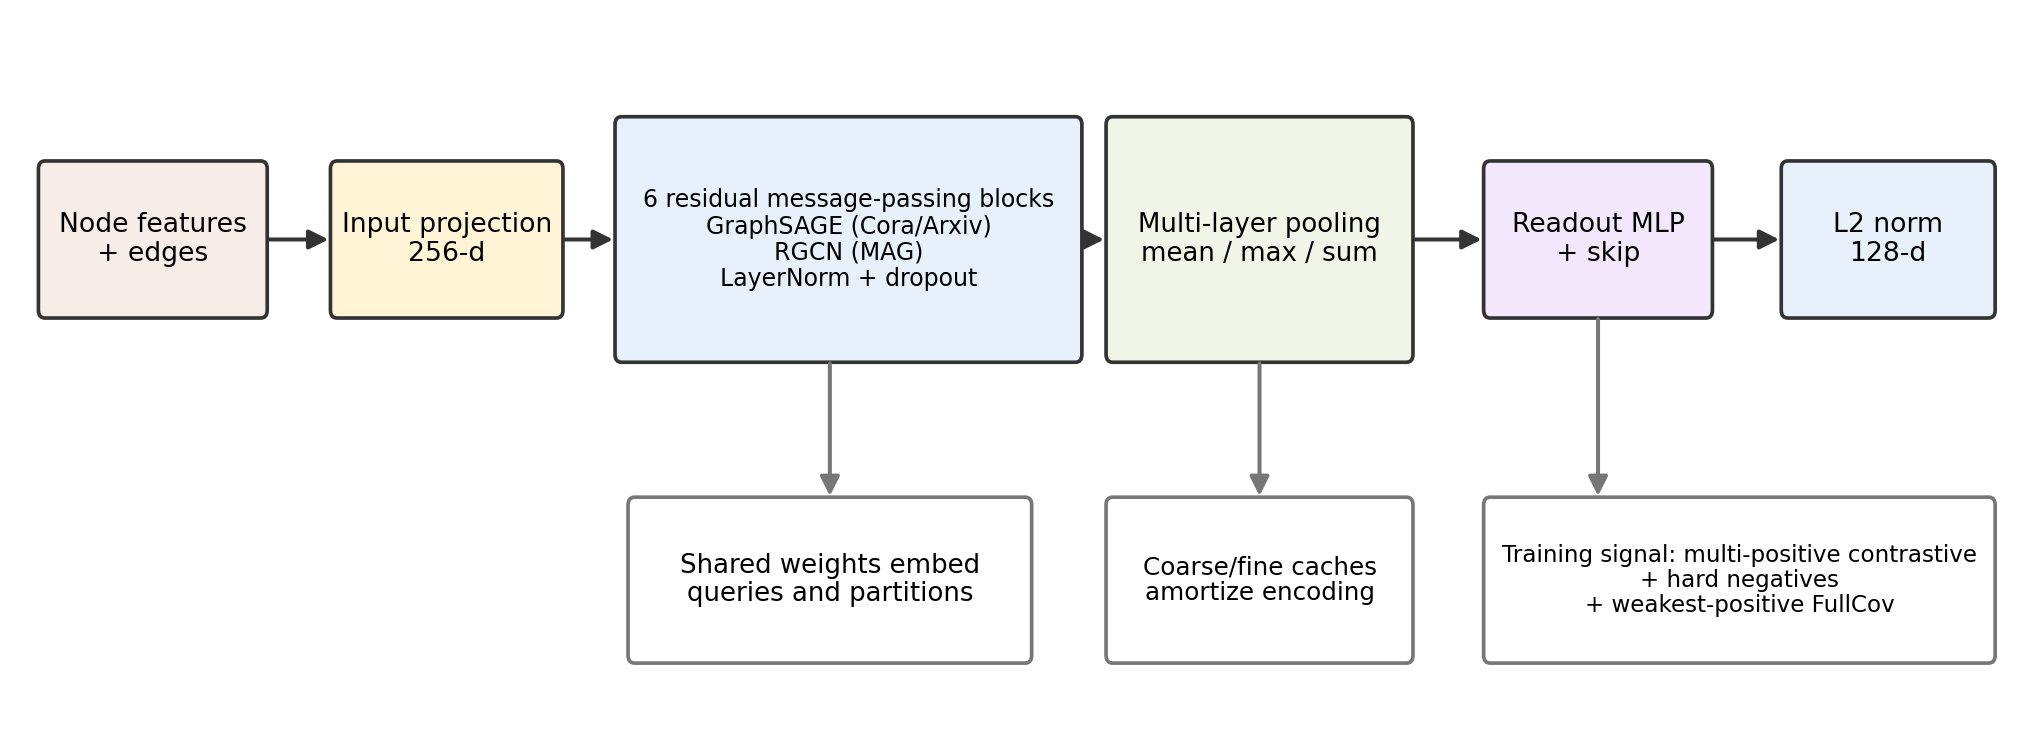
\includegraphics[width=\textwidth]{fig_encoder_architecture.png}
\caption{\textbf{Retrieval encoder.} Cora and Arxiv use a six-block residual GraphSAGE encoder; MAG uses the same six-block residual architecture with relation-aware RGCN layers. The same encoder embeds queries and cached graph partitions into a normalized 128-dimensional space.}
\label{fig:encoder}
\end{figure}

The encoder is intentionally shared between query graphs and partition graphs. Input node features are projected to a 256-dimensional hidden space, passed through six residual message-passing blocks, normalized with LayerNorm, and read out with multi-layer global mean, max, and sum pooling. The readout is an MLP plus a skip projection, followed by L2 normalization to produce a 128-dimensional retrieval vector. This matters because the retrieval problem is not node alignment; it is region localization. The model must place a query near every partition needed for exact verification, including the weakest or farthest true partition.

For Cora and Arxiv, the message-passing block is GraphSAGE ($\mathtt{SAGEConv}$); on these label-rich graphs a matched objective ablation finds GraphSAGE at least as strong as a GIN encoder at the fixed budgets the cascade uses, so we adopt it as the homogeneous-graph encoder. OGBN-MAG is a \emph{heterogeneous} academic graph (paper, author, institution, and field-of-study nodes joined by typed relations); we flatten it to a single node/edge index for the pipeline but \emph{retain} node types and relation (edge) types and model them with a relation-aware six-layer RGCN ($\mathtt{RGCNConv}$ with per-relation bases over $2R$ relations after symmetrization). Because OGBN-MAG supplies input features only on paper nodes, non-paper nodes receive node-type one-hot and per-relation-degree features, so the retriever reasons over typed structure rather than discarding it. Both encoders use the same retrieval interface: cached fine and coarse partition embeddings are compared to query embeddings, and positive partitions can be live-reencoded during training so coverage gradients update required positives instead of treating the entire partition bank as stale constants.

Training uses three complementary signals: multi-positive contrastive learning pulls a query toward all coarse partitions touched by the planted match; hard negatives keep nearby but incorrect partitions separated; and the FullCov-oriented coverage term penalizes the weakest required positive. In the final MAG training run, the selected checkpoint is the validation-best FullCov model rather than the final-epoch checkpoint; this is why the final benchmark bundle separates \texttt{mag\_rgcn\_best} production rows from \texttt{mag\_rgcn\_final} diagnostic rows.

\section{Partition Balance and Overlap Scale}
\label{app:partitions}

The hierarchy below is used by the corrected overlap-cascade artifacts. The overlap operator adds, for a selected partition $p$, only the \emph{boundary nodes} of other partitions that share an edge with $p$ -- not the entire bordering partitions. On MAG a median partition borders 948 of the 2{,}000 coarse partitions, but the boundary nodes it actually admits number only about 4{,}252; the expanded region for a single selected partition is therefore about 5{,}228 nodes (a $5.4\times$ expansion over the 969-node partition), not the $\approx$921K one would get by taking the union of every bordering partition in full. That 921K figure is a loose reachability bound the operator never realizes. Candidate size grows large only when the cascade \emph{unions} the boundary overlaps of the hundreds to a thousand partitions in the retrieval budget, and because boundary nodes are shared this union saturates at roughly 59--83\% of MAG at the largest budgets (59\% for Jigsaw, up to 83\% for uninformed policies). Overlap is thus a per-partition recall-expansion mechanism that is individually tight but collectively broad.

\begin{table}[h]
\centering
\caption{\textbf{Partition balance.} Coarse partitions are ranked by retrieval; fine partitions support local overlap and bridge construction. Node counts are per partition.}
\label{tab:partition_sizes}
\scriptsize
\resizebox{\textwidth}{!}{\begin{tabular}{llrrrrrrr}
\toprule
\textbf{Dataset} & \textbf{Level} & \textbf{Graph nodes} & \textbf{Parts} & \textbf{Min} & \textbf{Median} & \textbf{Mean} & \textbf{P90} & \textbf{Max} \\
\midrule
Cora & Coarse & 19,793 & 20 & 962 & 986 & 989.6 & 1,018 & 1,019 \\
Cora & Fine & 19,793 & 100 & 190 & 197 & 197.9 & 204 & 205 \\
Arxiv & Coarse & 169,343 & 200 & 822 & 846 & 846.7 & 872 & 872 \\
Arxiv & Fine & 169,343 & 1,000 & 153 & 169 & 169.3 & 175 & 195 \\
MAG & Coarse & 1,939,743 & 2,000 & 876 & 969 & 969.9 & 999 & 999 \\
MAG & Fine & 1,939,743 & 10,000 & 170 & 194 & 194.0 & 200 & 210 \\
\bottomrule
\end{tabular}
}
\end{table}

\begin{table}[h]
\centering
\caption{\textbf{Overlap expansion scale, stated precisely.} ``+Boundary overlap'' is the median number of boundary nodes the operator actually admits for one selected partition; ``Expanded part'' is partition plus boundary overlap (with the multiple over the bare partition). ``Neighbor parts'' counts the partitions a part borders. ``Loose union bound'' is the median size if one instead took every bordering partition in full -- a reachability bound the operator never realizes. The realized per-partition overlap is small ($5.4\times$ on MAG); breadth arises only from unioning over the retrieval budget.}
\label{tab:partition_overlap}
\footnotesize
\resizebox{\textwidth}{!}{\begin{tabular}{lrrrrrr}
\toprule
\textbf{Dataset} & \textbf{Coarse parts} & \shortstack{\textbf{Partition}\\\textbf{nodes (med)}} & \shortstack{\textbf{+Boundary}\\\textbf{overlap (med)}} & \shortstack{\textbf{Expanded part}\\\textbf{(med / $\times$)}} & \shortstack{\textbf{Neighbor parts}\\\textbf{med / max}} & \shortstack{\textbf{Loose union}\\\textbf{bound (med)}} \\
\midrule
Cora  & 20    & 986 & 534   & 1,533 / 1.6$\times$ & 18 / 19    & 18,820 \\
Arxiv & 200   & 846 & 1,606 & 2,470 / 2.9$\times$ & 135 / 173  & 115,004 \\
MAG   & 2,000 & 969 & 4,252 & 5,228 / 5.4$\times$ & 948 / 1,999 & 921,494 \\
\bottomrule
\end{tabular}
}
\end{table}

\begin{figure}[h]
\centering
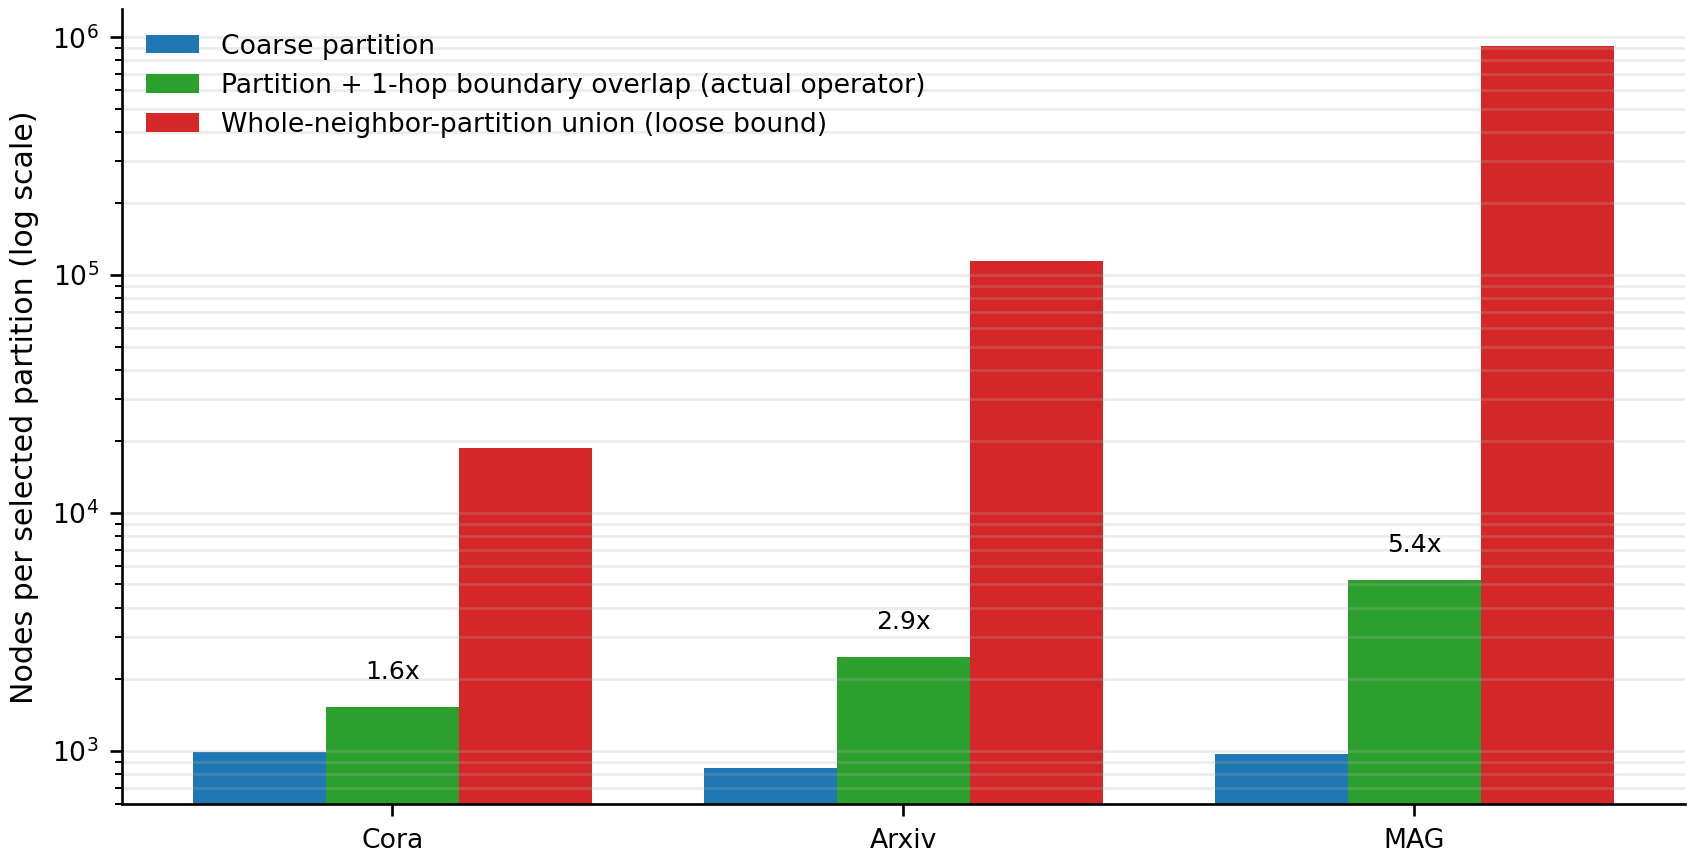
\includegraphics[width=0.82\textwidth]{fig_partition_overlap_stats.png}
\caption{\textbf{What one selected partition actually contributes (log scale).} The realized one-hop boundary overlap (green) expands a coarse partition only modestly ($1.6\times$ on Cora, $2.9\times$ on Arxiv, $5.4\times$ on MAG). The red bar is the loose union-of-whole-neighbor-partitions bound that the operator never realizes; reporting it as ``the overlap'' overstates MAG breadth by more than $170\times$. Candidate breadth instead comes from unioning these tight per-partition overlaps across the retrieval budget.}
\label{fig:partition_overlap}
\end{figure}

\section{Query-Family Breakdown and Budget Curves}
\label{app:family}

\begin{table}[h]
\centering
\caption{\textbf{Jigsaw query-family breakdown.} Positive columns report exact-solve rate; negative columns report correct no-match rate. All three datasets use the corrected connected multi-family reruns. All datasets are reported at the matched half-partition budget ($K{=}10/100/1000$); the MAG rows use the deployed walk-aware encoder (overall $88.6\%$).}
\label{tab:jigsaw_family}
\scriptsize
\setlength{\tabcolsep}{3pt}
\resizebox{\textwidth}{!}{%
\begin{tabular}{lrrrrrrrr}
\toprule
\textbf{Dataset} & \textbf{Single} & \textbf{K-hop} & \textbf{Deg-K} & \textbf{Walk} & \textbf{Multi-fine} & \textbf{Multi-coarse} & \textbf{Neg-label} & \textbf{Neg-struct} \\
\midrule
Cora & 100.0 & 98.3 & 97.3 & 75.3 & 100.0 & 94.3 & 100.0 & 100.0 \\
Arxiv & 100.0 & 97.3 & 98.3 & 82.3 & 100.0 & 78.7 & 100.0 & 100.0 \\
MAG & 98.7 & 93.3 & 92.7 & 71.0 & 100.0 & 76.0 & 100.0 & 99.7 \\
\bottomrule
\end{tabular}}
\end{table}

The query-family view explains the aggregate rates. At the matched half-partition budget the \emph{same} family pattern holds across all three datasets: single and multi-fine saturate, local K-hop families remain high but not perfect on MAG (K-hop $93.3\%$, degree K-hop $92.7\%$), and random-walk and multi-coarse are hardest everywhere (random-walk $75.3/82.3/71.0\%$, multi-coarse $94.3/78.7/76.0\%$ on Cora/Arxiv/MAG) -- hard families are intrinsic to the query type, not graph scale. MAG preserves high single (98.7\%) and local K-hop recovery, and its multi-region families also solve well (multi-fine 100\%, multi-coarse 76.0\%); the one family that stays hardest is random walks (71.0\%).

The random-walk weakness is the most instructive single failure, and it is the same mechanism as the wasted-overlap finding in Section~\ref{sec:shrinkage}. It is \emph{not} a solver problem: FilterAll solves random walks at 96.0\%, and 96.6\% of Jigsaw's random-walk failures occur before the solver, with the planted match never entering the candidate. It is also not partition count: random walks span about as many coarse partitions as K-hop queries (median 29 vs 23). The discriminator is overlap recovery. A K-hop query is a compact BFS ball, so a missed partition's nodes sit on the boundary of retrieved partitions and one-hop overlap recovers it 94\% of the time. A random walk is a diffuse path whose missed mid-path partitions are typically not boundary-adjacent to any retrieved partition, so overlap recovers only 62\% of misses, and a single unrecovered node forfeits the match. The effect scales with walk length (deployed walk-aware solve $0.94\!\to\!0.40$ from size 20 to 100) and with graph size -- it is far milder on the smaller, denser Arxiv (random-walk $82.3\%$ at the half-partition budget, reaching $100\%$ only by the full $200$-partition budget) and severe only at MAG scale. This is precisely the family where the learned retriever has its clearest edge over Mean-RRF ($+10$ points on this family, $+15$ points at size 100), because better partition ranking is the one lever that helps once overlap cannot stitch the gaps.

An overlap-side remedy is structurally unpromising: on MAG's high-degree coarse quotient graph a partition borders a median 948 of 2{,}000 others, so a missed mid-walk partition cannot be singled out from hundreds of equally-connected neighbors without re-admitting much of the graph. We therefore conclude the random-walk bottleneck is genuinely \emph{retrieval ranking}, not overlap construction; and this holds at fine granularity too---a fine partition still borders a mean $568$ of $10{,}000$---so the inference-time remedies catalogued in Appendix~\ref{app:probes} do not close the gap. The deployed MAG encoder is trained with exactly this walk-aware objective (a random-walk- and multi-coarse-weighted distribution of larger $50$--$100$-node queries) on a training query stream (training seed 7203) \emph{disjoint} from the held-out evaluation seeds (20260607/08), so every reported walk-aware number is on queries never seen in training --- the retrain reshaped the training \emph{distribution}, not the test set: relative to a generic-mix encoder (which reaches $86.0\%$ overall, random-walk only $60.0\%$, multi-coarse $71.7\%$), it lifts random-walk to $71.0\%$ and multi-coarse to $76.0\%$ -- hence overall MAG to the \textbf{88.6\%} of Table~\ref{tab:production_matrix} -- with no meaningful regression on the easy families (single $99.3\!\to\!98.7$, within noise). The paired McNemar confirms the gain: across all $1800$ positives walk-aware Jigsaw beats Mean-RRF $92$ to $35$ (exact $p{=}4.4{\times}10^{-7}$), the advantage concentrated in these two hard families (multi-coarse $34/12$, random-walk $44/13$; the remaining families contribute $14/10$ and are statistically tied).

The cumulative solved-by-budget curves are explicit in the release CSVs. With the overlap-aware retrievers, Jigsaw's cumulative solve rises $64.0/82.7/94.2/100$ on Cora (budgets 2/5/10/20), $69.6/81.3/92.8/100$ on Arxiv (20/50/100/200), and $37.6/46.0/53.0/61.9/75.4/88.6$ on MAG (20/50/100/200/500/1000) with the deployed walk-aware encoder; read at the half-partition budget Jigsaw solves $94.2/92.8/88.6$ on Cora/Arxiv/MAG. The $100\%$ Cora/Arxiv figures require every partition and are the exhaustive ceiling. MAG's per-size slices at $K{=}1000$ are 93.2/90.7/82.0 for sizes 20/50/100.

\begin{figure}[h]
\centering
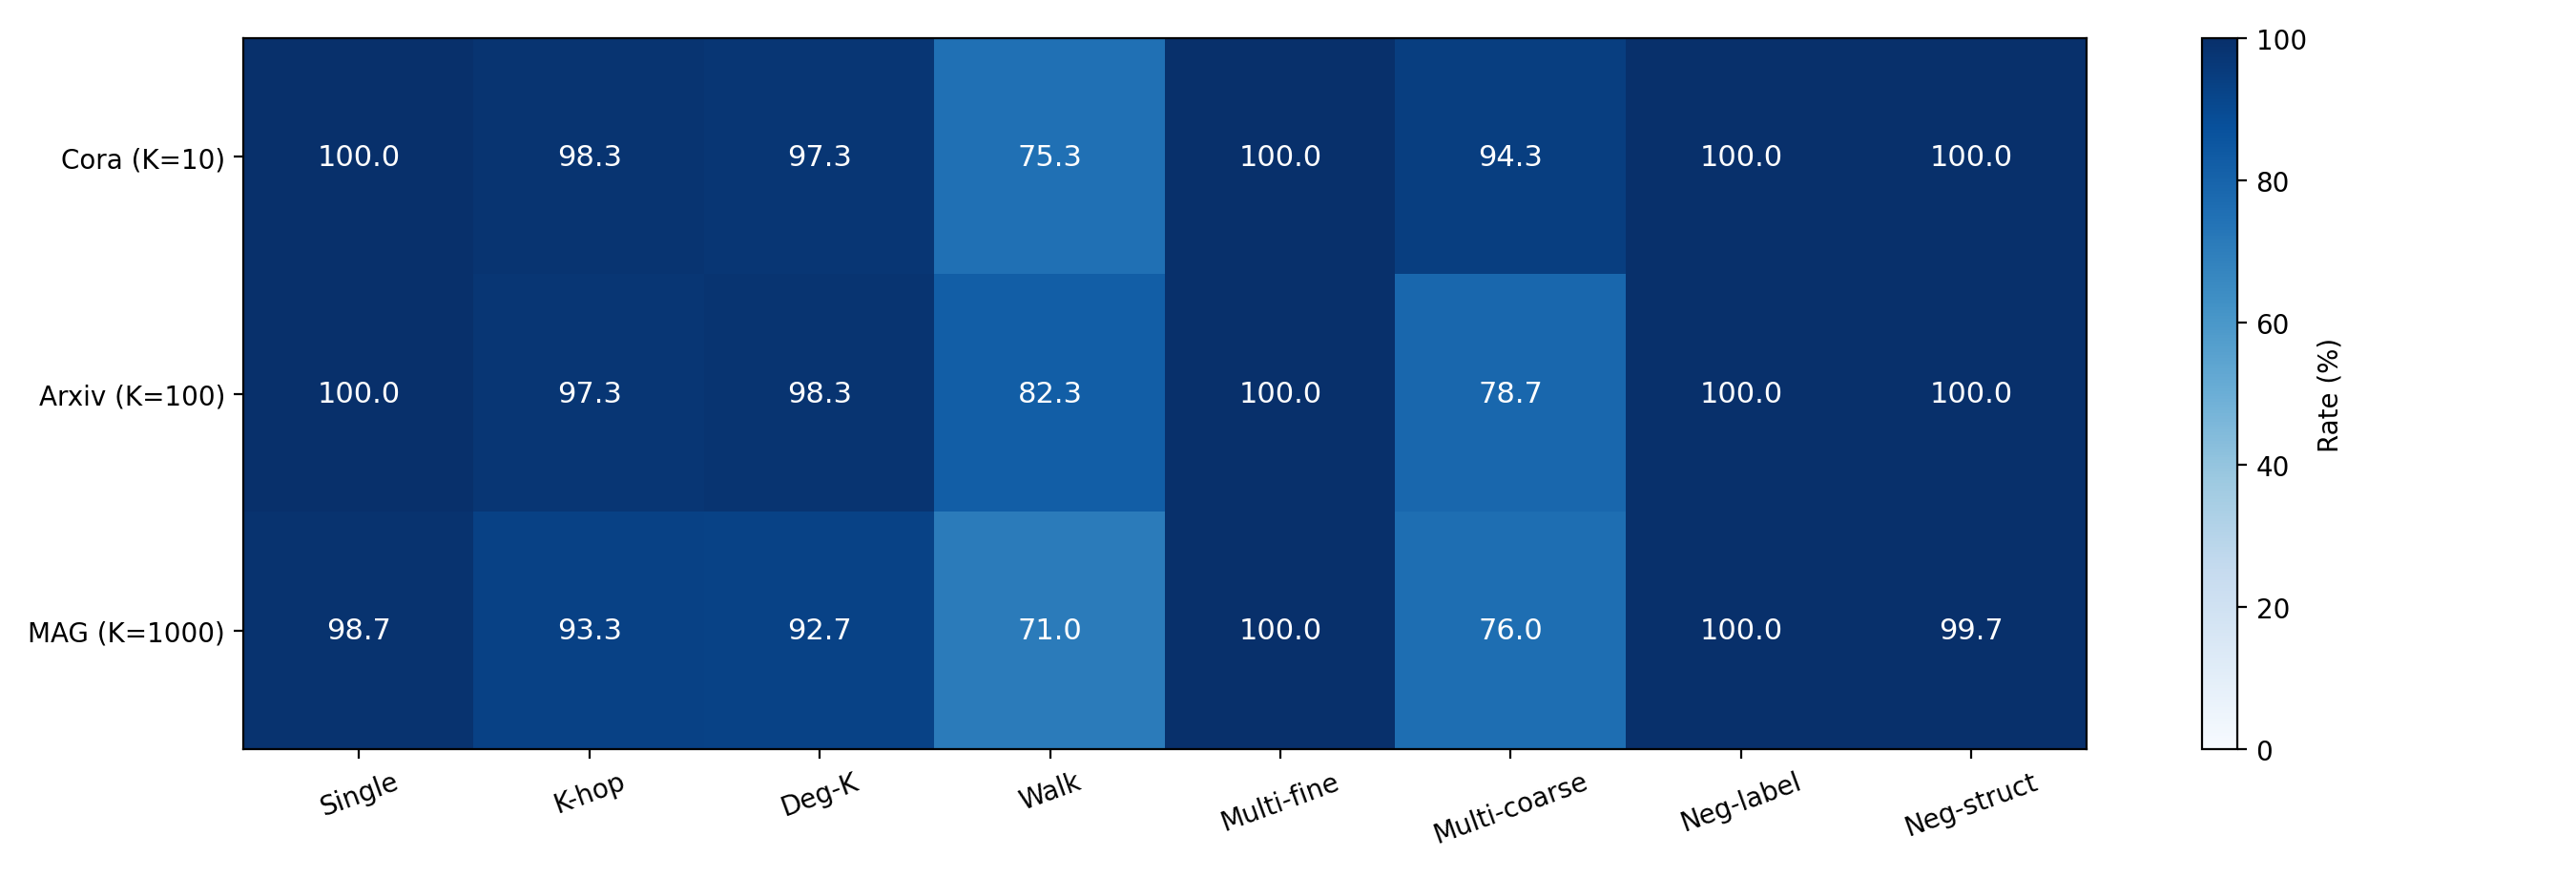
\includegraphics[width=\textwidth]{fig_jigsaw_query_family_heatmap.png}
\caption{\textbf{Jigsaw query-family outcomes.} Positive families report exact-solve rate; negative families report correct no-match rate. All rows are at the matched half-partition budget ($K{=}10/100/1000$). Random-walk and multi-coarse are the hard families across \emph{all three} datasets (Walk $75/82/71\%$, Multi-coarse $94/79/76\%$); single and multi-fine templates saturate, while local K-hop variants remain high but not perfect on MAG.}
\label{fig:query_family_heatmap}
\end{figure}

\begin{figure}[h]
\centering
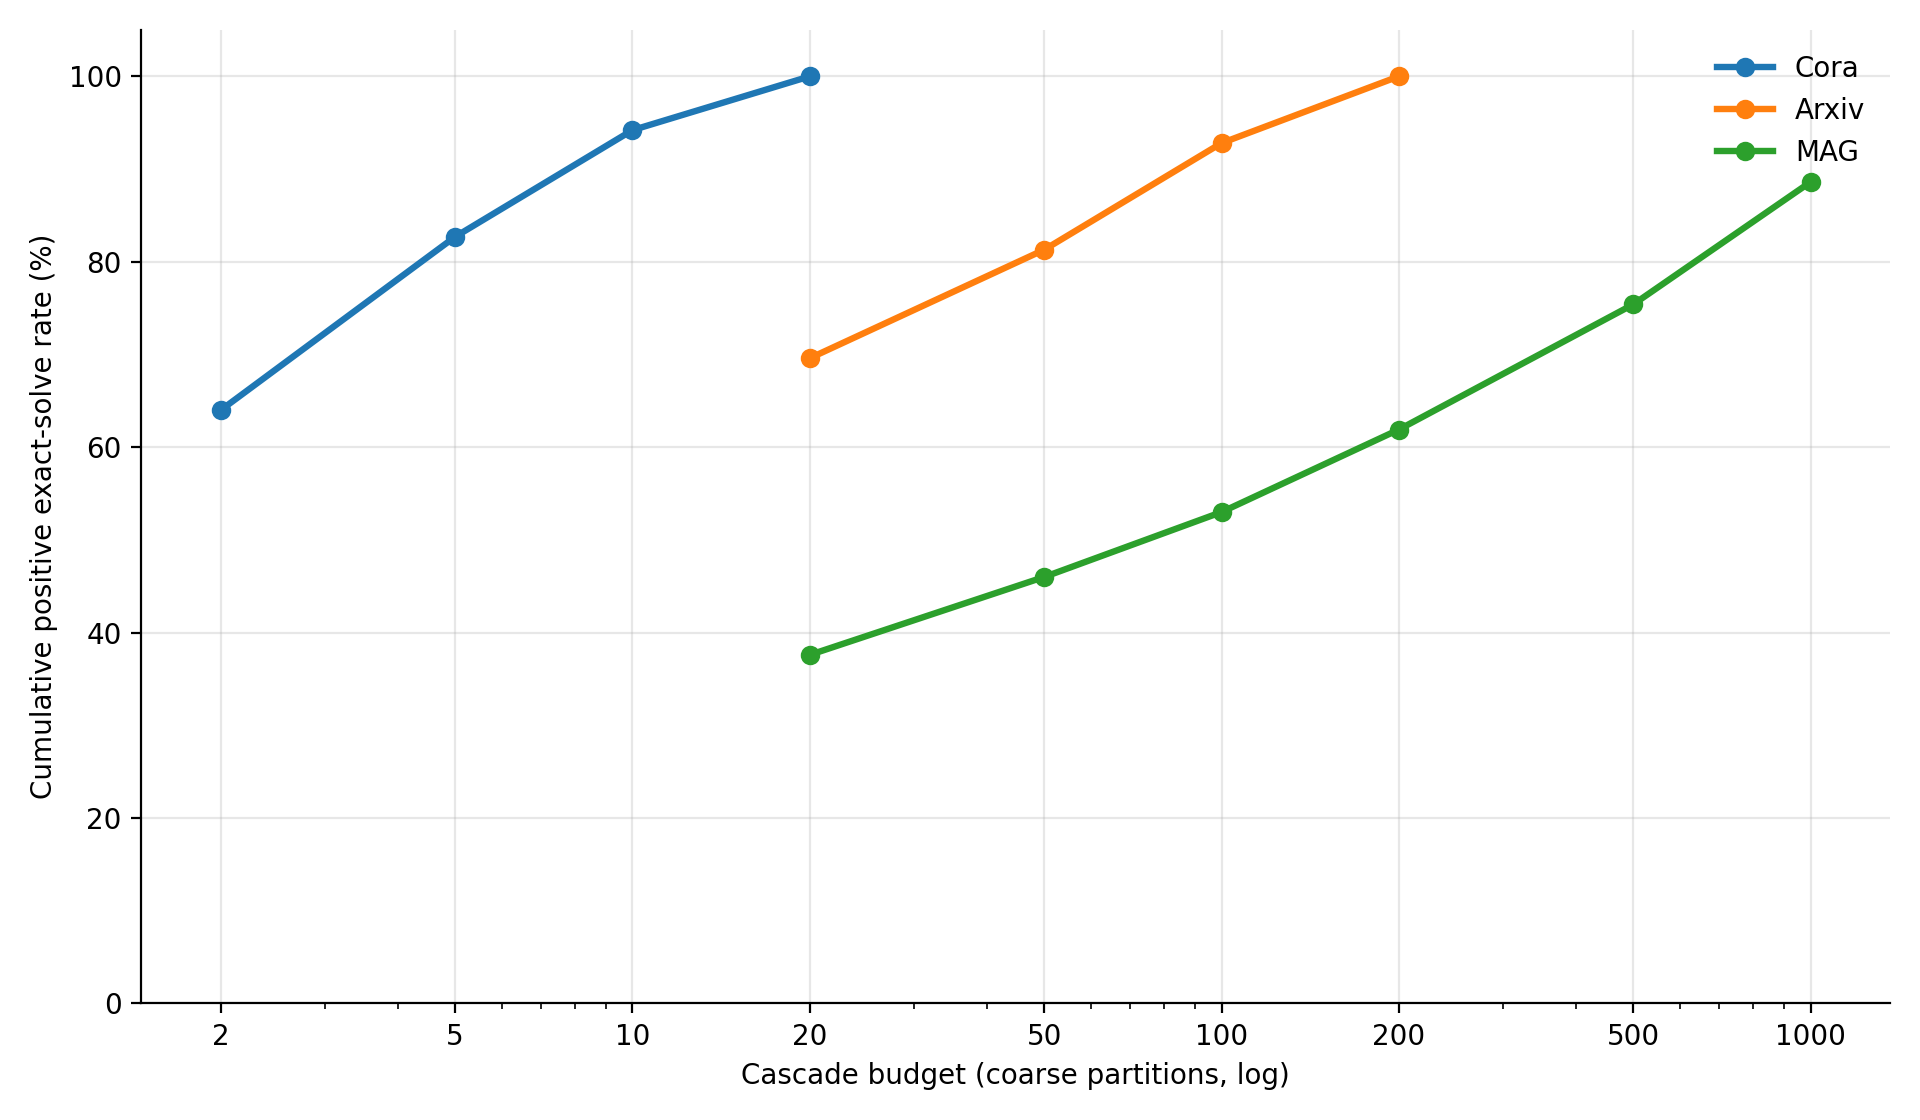
\includegraphics[width=0.80\textwidth]{fig_jigsaw_budget_curves.png}
\caption{\textbf{Solved-by-budget curves for Jigsaw.} Cora solves early because its candidate graphs are small and labels are strong. Arxiv benefits from budget expansion through 200. MAG continues improving through 1000, reflecting larger candidate regions and harder coverage.}
\label{fig:budget_curves}
\end{figure}

On Cora the curve rises steeply ($64.0\%$ at budget 2 to $100\%$ by budget 20), so a handful of partitions decides most queries. Arxiv needs budget expansion to 200 before reaching its final positive solve rate, even though all policies eventually reach 100\%. MAG continues to improve through 500 and 1000, which means failures at small budgets are often not verifier unsoundness but insufficient candidate expansion. This supports exposing budget as a control knob rather than using one fixed candidate size for all queries.

\section{System-Design Ablations and Model-Variant Diagnostics}
\label{app:design}

\begin{table}[h]
\centering
\caption{\textbf{Operator-necessity ablation (shared 48-query set per dataset).} Each row disables one cascade operator on one shared query set; rows measure \emph{relative} necessity, so absolute rates are diagnostic. The datasets stress \emph{different} operators: on MAG, removing \textbf{overlap} halves the positive solve rate (boundary-crossing matches cannot complete); on Arxiv (all variants still solve $100\%$) removing \textbf{signatures} explodes the candidate domain ${\sim}75\times$ ($94{\to}7{,}081$). Overlap is a no-op on Arxiv and signatures are inert on MAG.}
\label{tab:design_ablation}
\scriptsize
\setlength{\tabcolsep}{5pt}
\resizebox{\textwidth}{!}{%
\begin{tabular}{lrrrr}
\toprule
 & \multicolumn{2}{c}{\textbf{OGBN-MAG}} & \multicolumn{2}{c}{\textbf{OGBN-Arxiv}} \\
\cmidrule(lr){2-3}\cmidrule(lr){4-5}
\textbf{Variant} & \textbf{Solve \%} & \textbf{Cand.} & \textbf{Solve \%} & \textbf{Cand.} \\
\midrule
Full Jigsaw    & 88.9          & 64.0K & 100.0 & 94 \\
No overlap     & \textbf{44.4} & 49.9K & 100.0 & 97 \\
No signature   & 88.9          & 64.0K & 100.0 & \textbf{7{,}081} \\
No components  & 63.9          & 65.2K & 100.0 & 94 \\
No exact-label & 52.8          & 100.7K  & 100.0 & 223 \\
\bottomrule
\end{tabular}}
\end{table}

\begin{figure}[h]
\centering
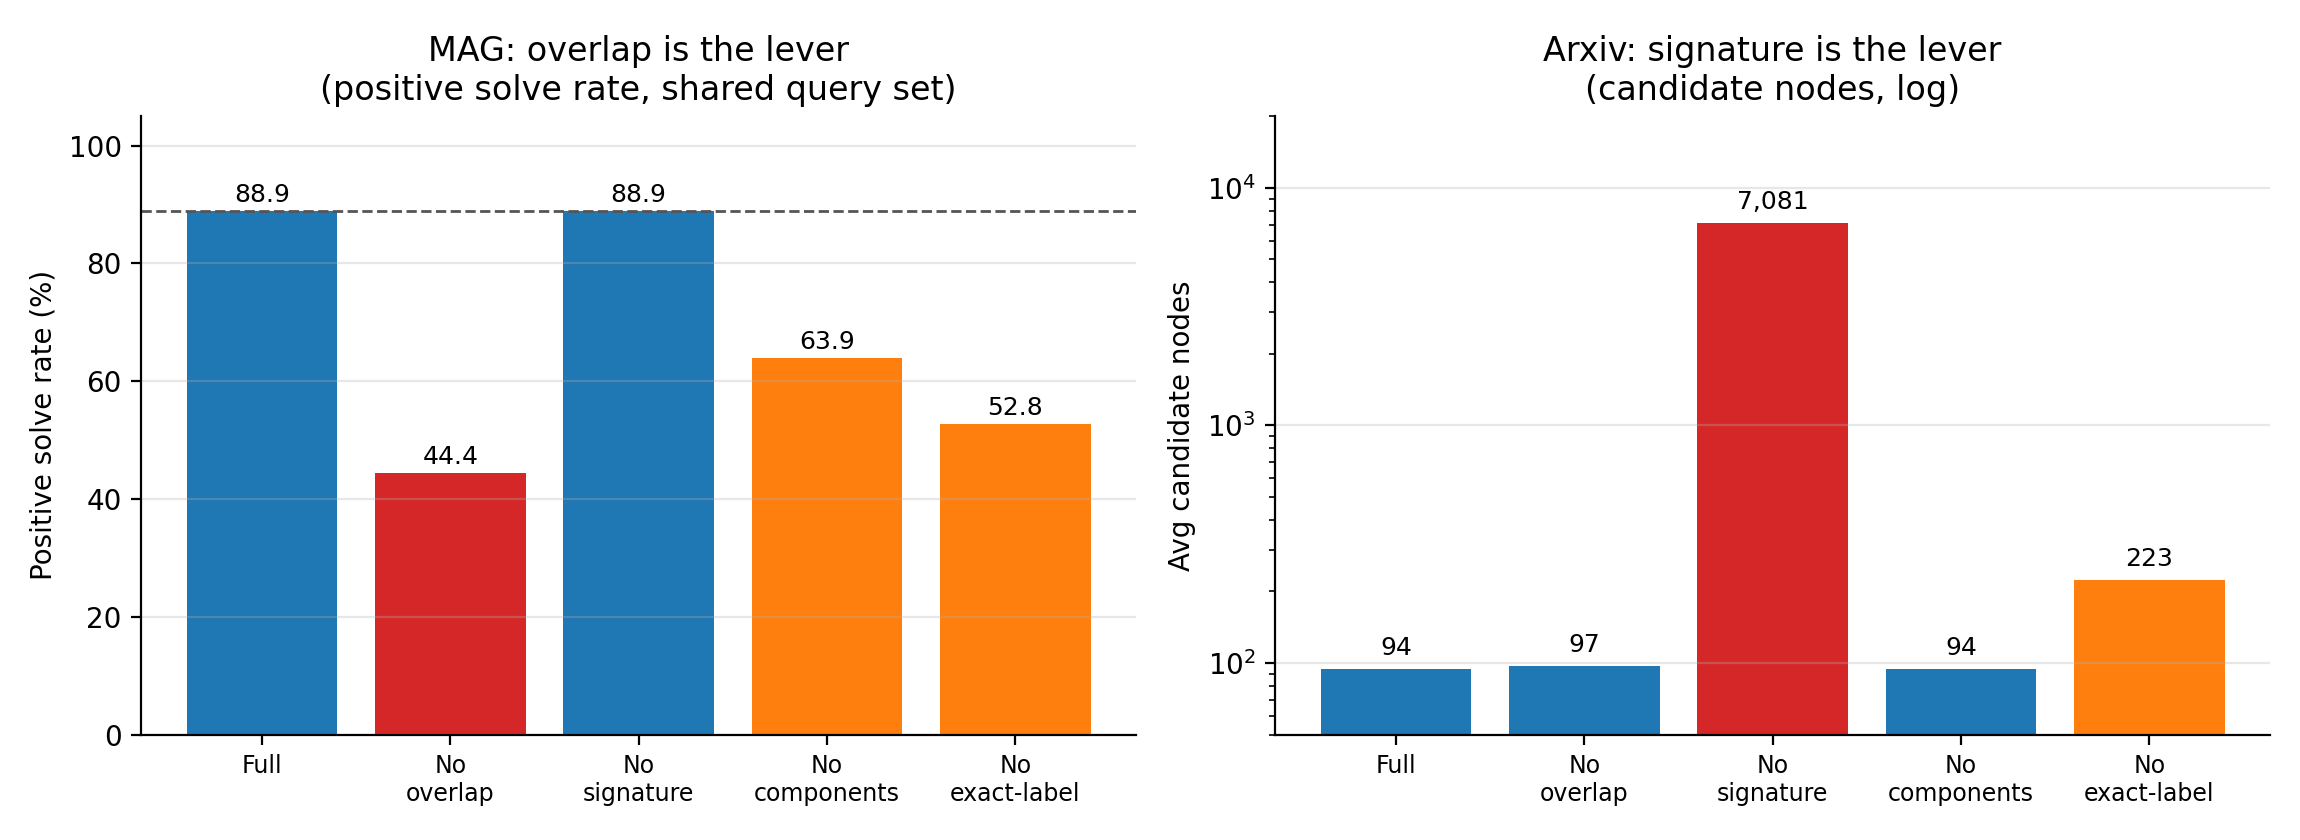
\includegraphics[width=0.78\textwidth]{fig_design_ablation.png}
\caption{\textbf{Operator necessity is dataset-dependent.} \emph{Left:} on MAG, disabling overlap halves the solve rate ($88.9{\to}44.4\%$); signatures are inert. \emph{Right:} on Arxiv, disabling signatures explodes candidates ${\sim}75\times$ ($94{\to}7{,}081$, log axis) while overlap is a no-op.}
\label{fig:design_ablation}
\end{figure}

The two ablations tell one story: the cascade's operators are \emph{dataset-dependent}, and both are necessary because different graphs stress different ones. On MAG (2{,}000 partitions, boundary-crossing queries) \textbf{overlap} is the pillar -- removing the one-hop halo halves the solve rate ($88.9{\to}44.4\%$) -- while signatures are inert (identical $88.9\%$ / $64.0$K), the flattened heterogeneous graph giving the typed fingerprint little to discriminate. On Arxiv the roles invert: overlap is a no-op ($94{\to}97$ candidate nodes) while \textbf{signatures} are the pillar, removing them inflating candidates ${\sim}75\times$ ($94{\to}7{,}081$) -- the explosion an exact verifier cannot afford at scale even when the small graph still solves. Exact-label pruning matters for candidate size and negatives (Arxiv $94{\to}223$; MAG solve $88.9{\to}52.8\%$), and component decomposition helps the MAG solve rate ($88.9{\to}63.9\%$). No single operator can be dropped: the one idle on one dataset is decisive on another. The Arxiv retrieval ablation (Table~\ref{tab:loss_ablation}) establishes the learning contribution; this establishes the systems contribution.

\paragraph{Model-variant diagnostics.}
The final benchmark bundle also preserves diagnostic rows not counted in the canonical production matrix. For Arxiv, continuation/v7 rows show that extending training can change retrieval behavior, but the selected production claim uses the base \texttt{arxiv} model for a balanced two-seed matrix. For MAG, both \texttt{mag\_rgcn\_best} and \texttt{mag\_rgcn\_final} were benchmarked; the production matrix uses \texttt{mag\_rgcn\_best} because validation selected it by FullCov, while \texttt{mag\_rgcn\_final} rows are retained as diagnostic model ablations rather than silently averaged into production.

\section{Additional Production Figures}
\label{app:figures}

\begin{figure}[h]
\centering
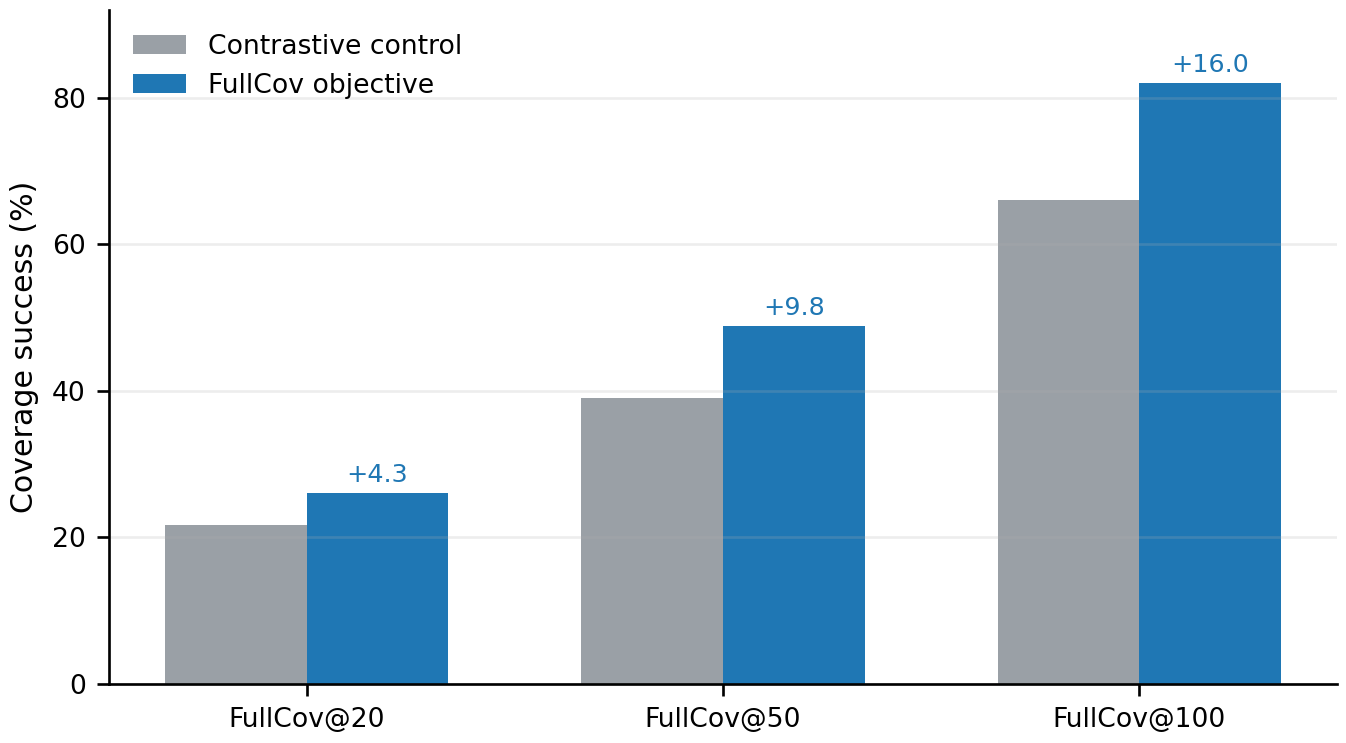
\includegraphics[width=0.72\textwidth]{fig_fullcov_ablation.png}
\caption{\textbf{FullCov objective gain.} Under matched Arxiv K-hop training conditions, directly optimizing weakest-positive coverage improves every fixed retrieval budget used by the downstream cascade.}
\label{fig:fullcov_ablation}
\end{figure}

\begin{figure}[h]
\centering
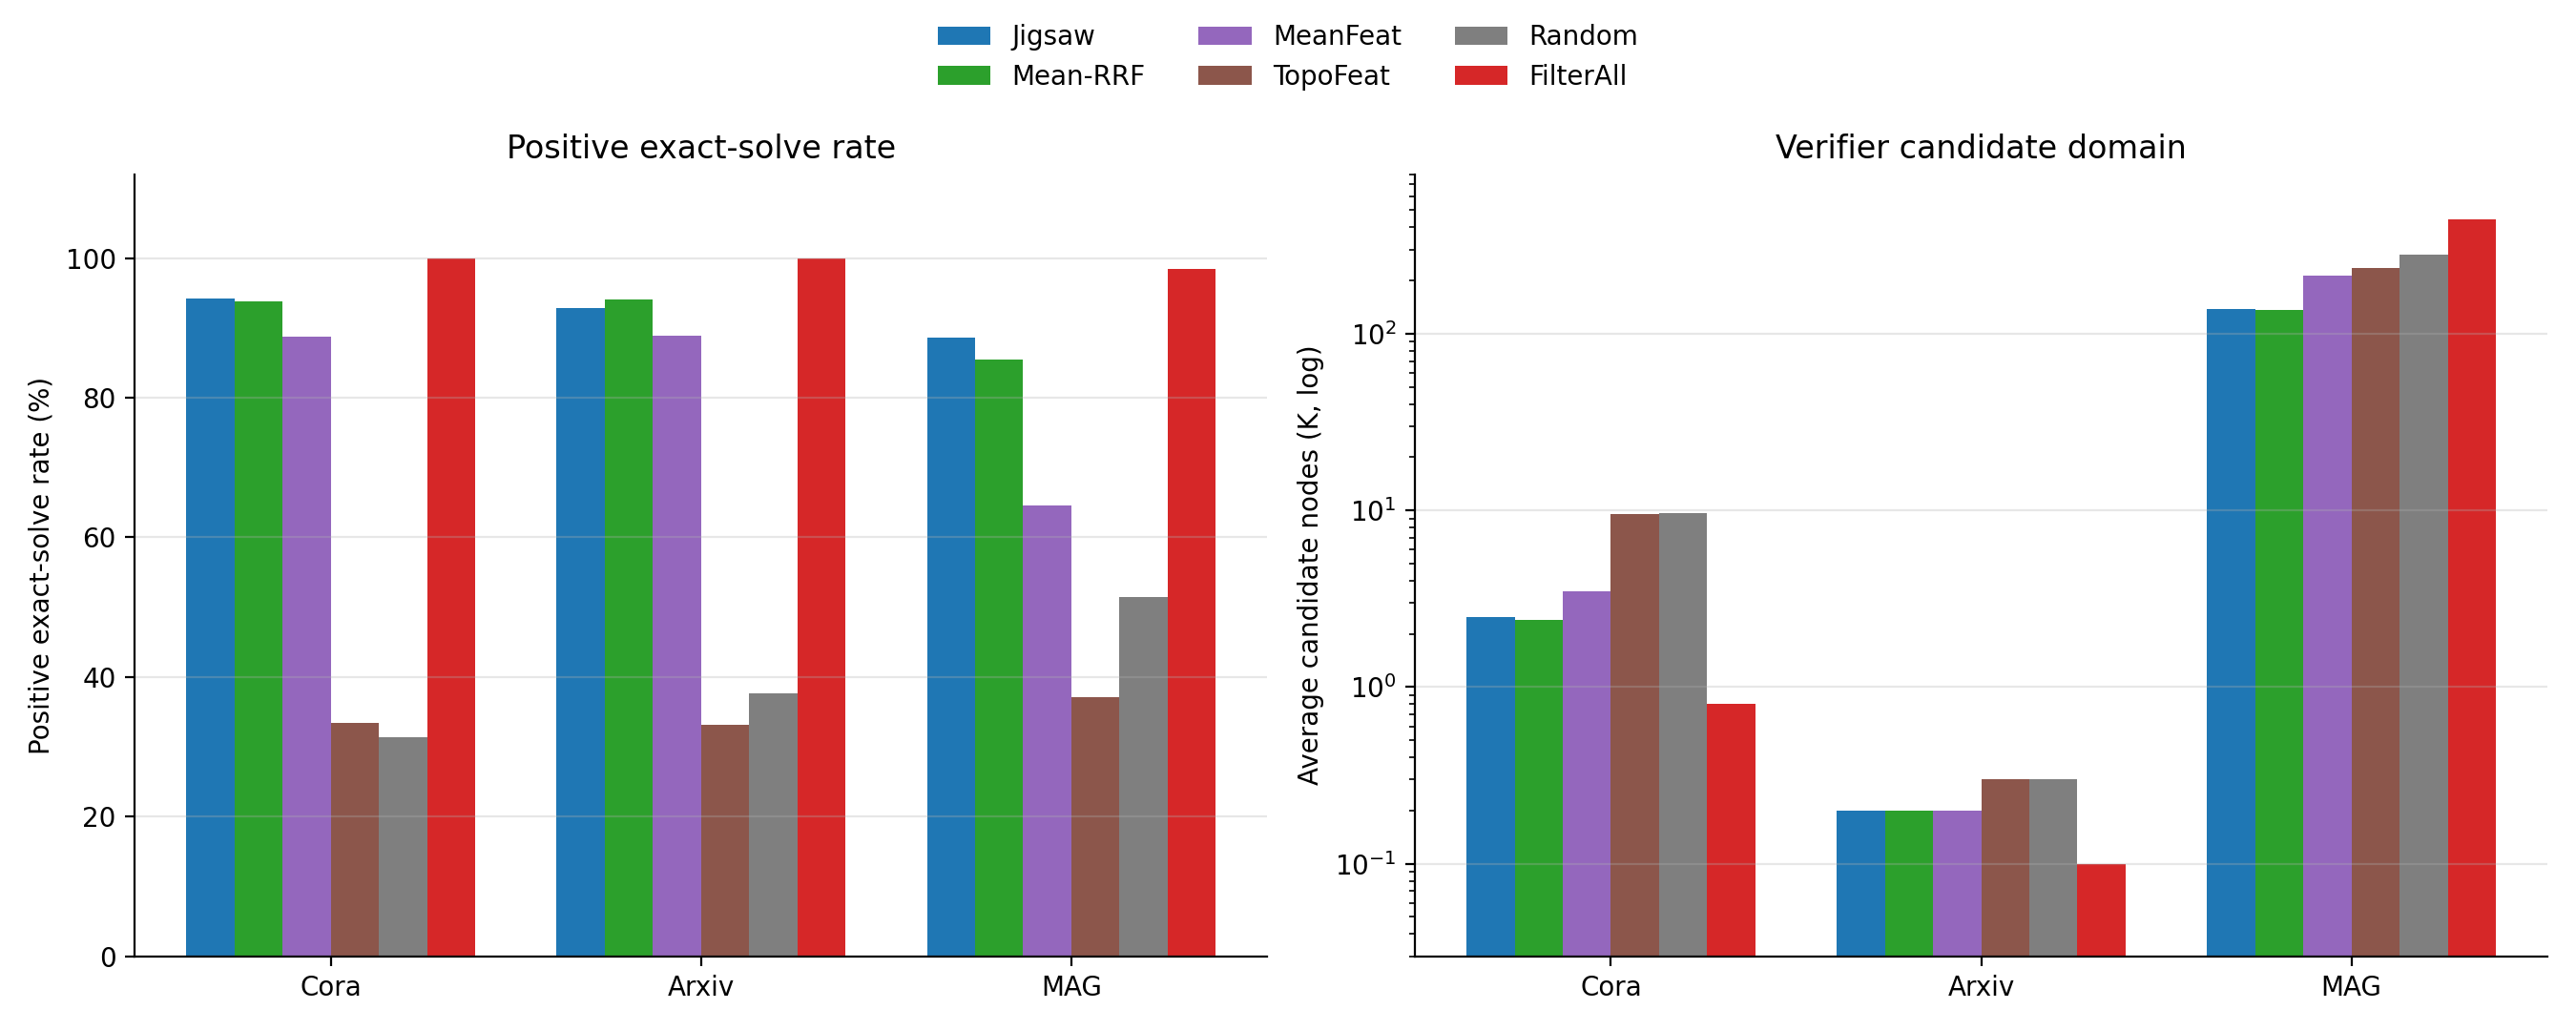
\includegraphics[width=\textwidth]{fig_production_positive_rates.png}
\caption{\textbf{Production positive exact-solve rates and candidate cost.} Production positive exact-solve rates at the matched half-partition budget ($K{=}10/100/1000$) and candidate cost. At this budget the policies separate on \emph{all three} datasets (random/topology fall to $31$--$51\%$: $31$--$38\%$ on Cora/Arxiv, $37$--$51\%$ on MAG); FilterAll (exhaustive, all partitions) is the ceiling that reaches $100\%$ on Cora/Arxiv. Right panel: verifier candidate domain (per-query average nodes).}
\label{fig:production_rates}
\end{figure}

\begin{figure}[h]
\centering
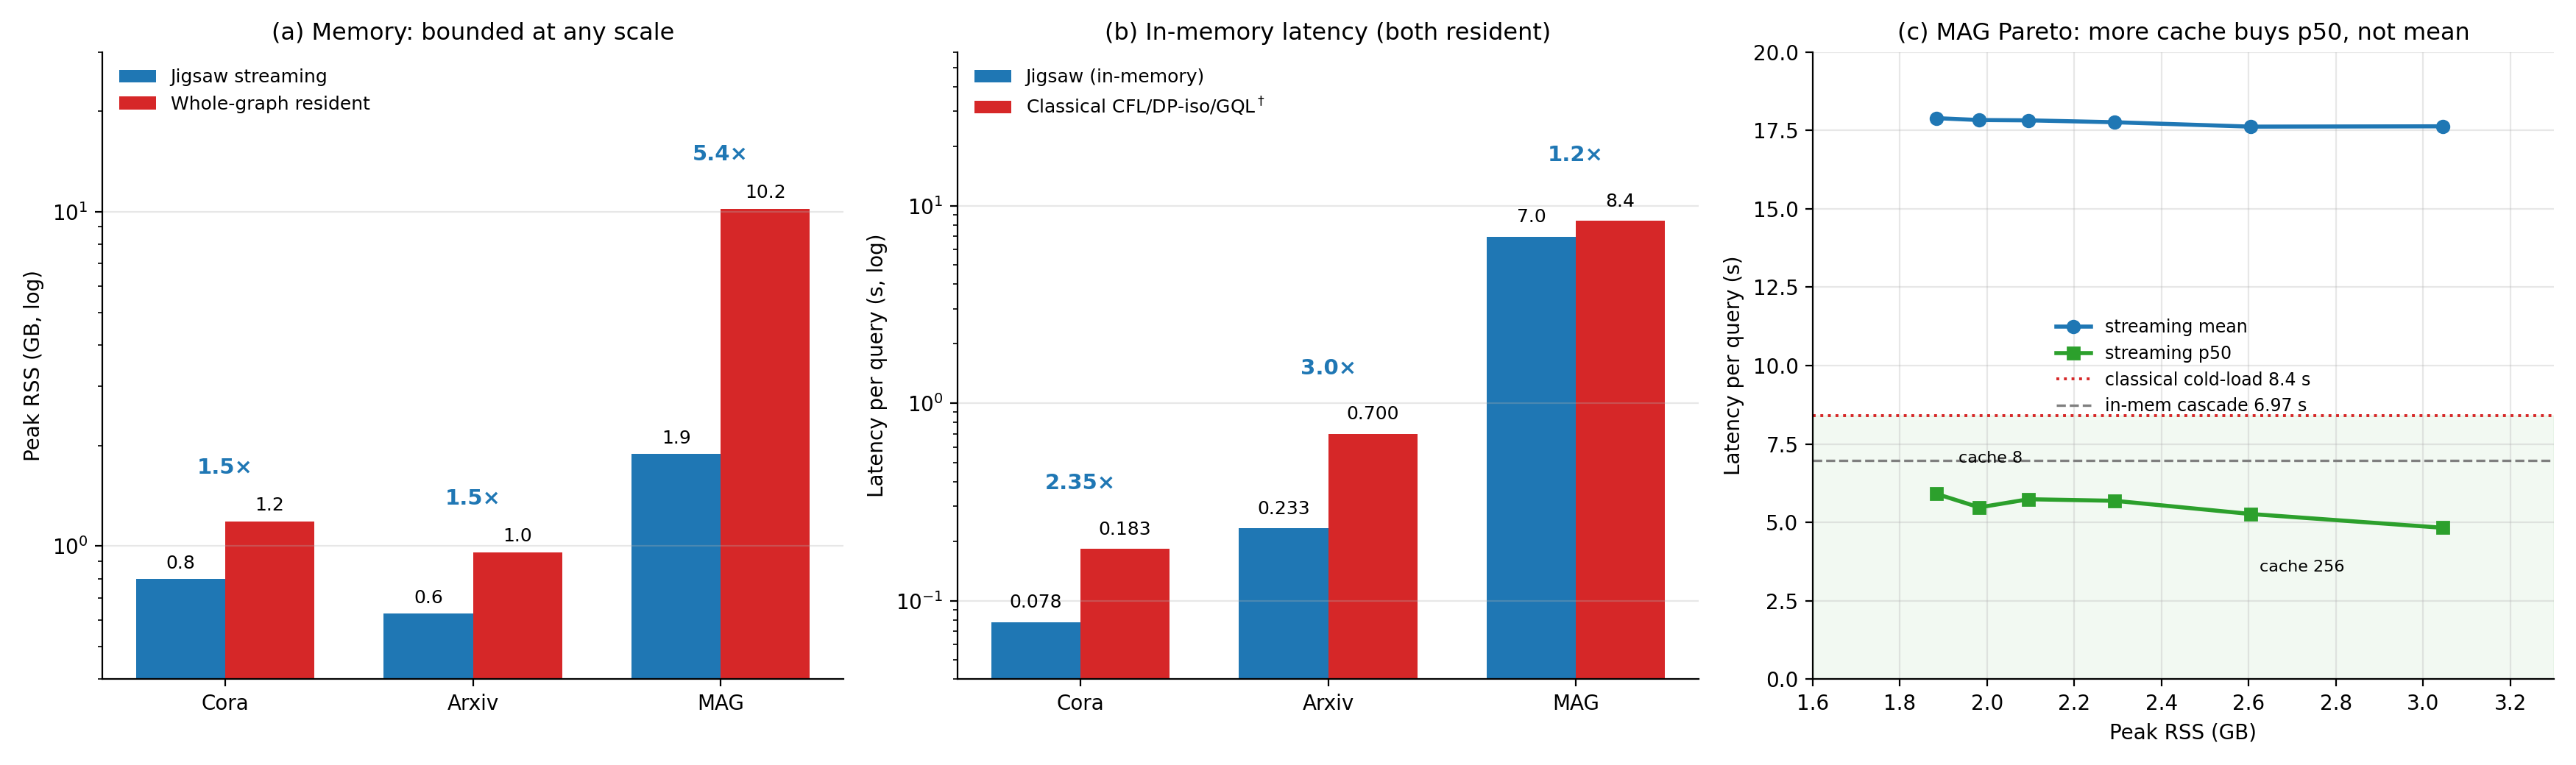
\includegraphics[width=\textwidth]{fig_memory_latency.png}
\caption{\textbf{Memory is the clean win; cold-load latency is competitive but load-dominated; the tradeoff is tunable.} \textbf{(a)} Streaming vs.\ whole-graph-resident peak RSS -- bounded on every dataset, $5.4\times$ smaller on MAG ($1.9$ vs $10.2$\,GB). \textbf{(b)} Cold-load end-to-end latency, Jigsaw vs.\ classical CFL/DP-iso/GQL: $2.35$/$3.0$/$1.2\times$ faster on Cora/Arxiv/MAG -- load avoidance, not faster resident matching ($^\dagger$MAG classical is cold per-query load, ${\sim}1$\,ms if resident), so no raw-speed claim. \textbf{(c)} MAG memory$\leftrightarrow$latency frontier as the cache grows ($8{\to}256$): more memory buys down p50 ($5.9{\to}4.8$\,s, below the $8.4$\,s cold-load) but the mean stays flat ($17.9{\to}17.6$\,s), a hard-query I/O tail not cache re-reads. Jigsaw lets the operator choose a frontier point an all-or-nothing resident matcher cannot. (The $2.4$\,GB in the body is the $8$-partition serve pre-vectorization; optimized it is $1.9$\,GB.)}
\label{fig:memory_latency}
\end{figure}

\begin{figure}[h]
\centering
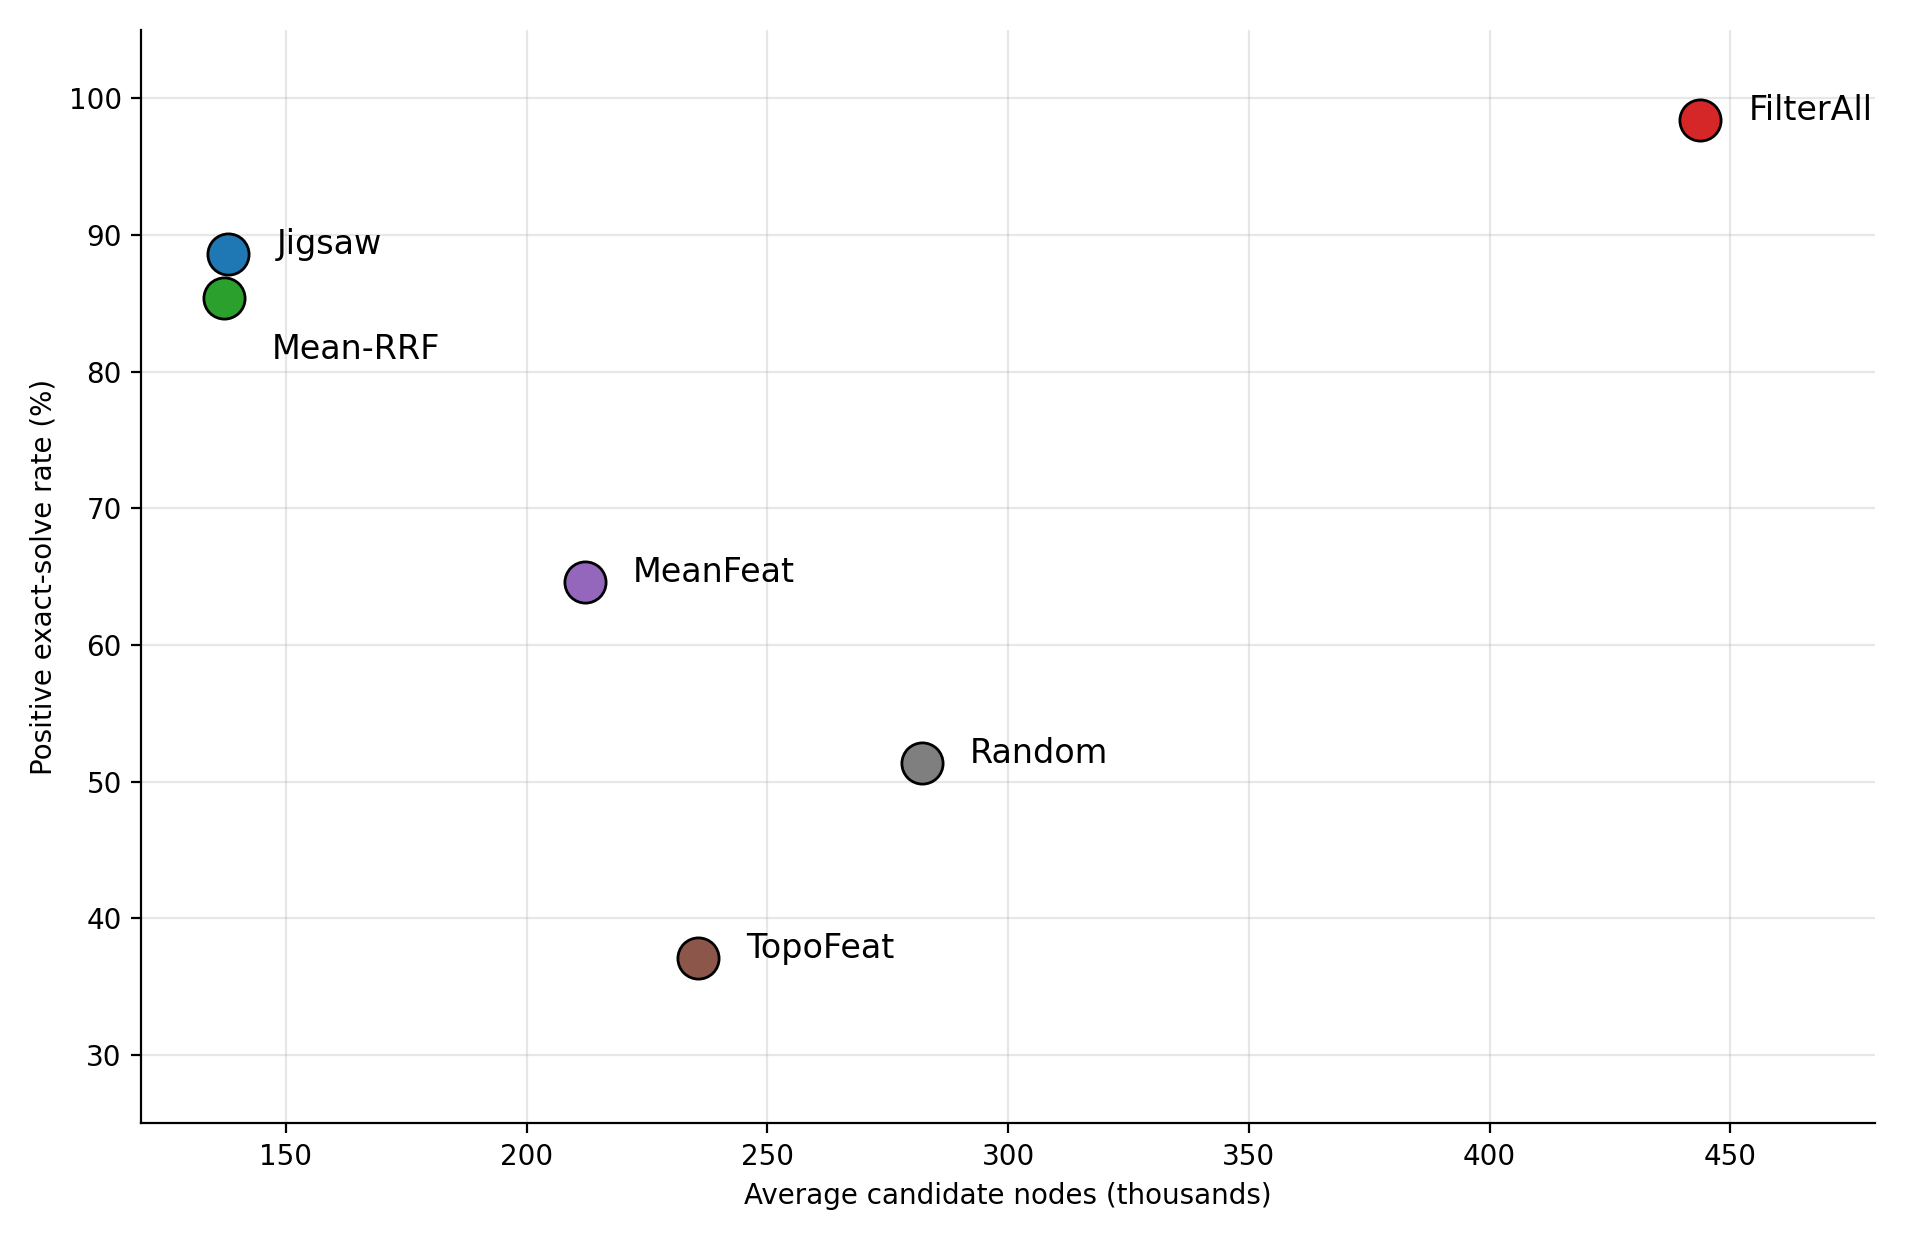
\includegraphics[width=0.86\textwidth]{fig_mag_tradeoff.png}
\caption{\textbf{MAG tradeoff.} MAG is the production dataset where retrieval policies separate sharply. FeatureIndex is strongest under near-unique labels; FilterAll is the exhaustive ceiling; learned Jigsaw is a memory-bounded operating point that uses less than half the candidate nodes of FilterAll.}
\label{fig:mag_tradeoff}
\end{figure}

\begin{figure}[h]
\centering
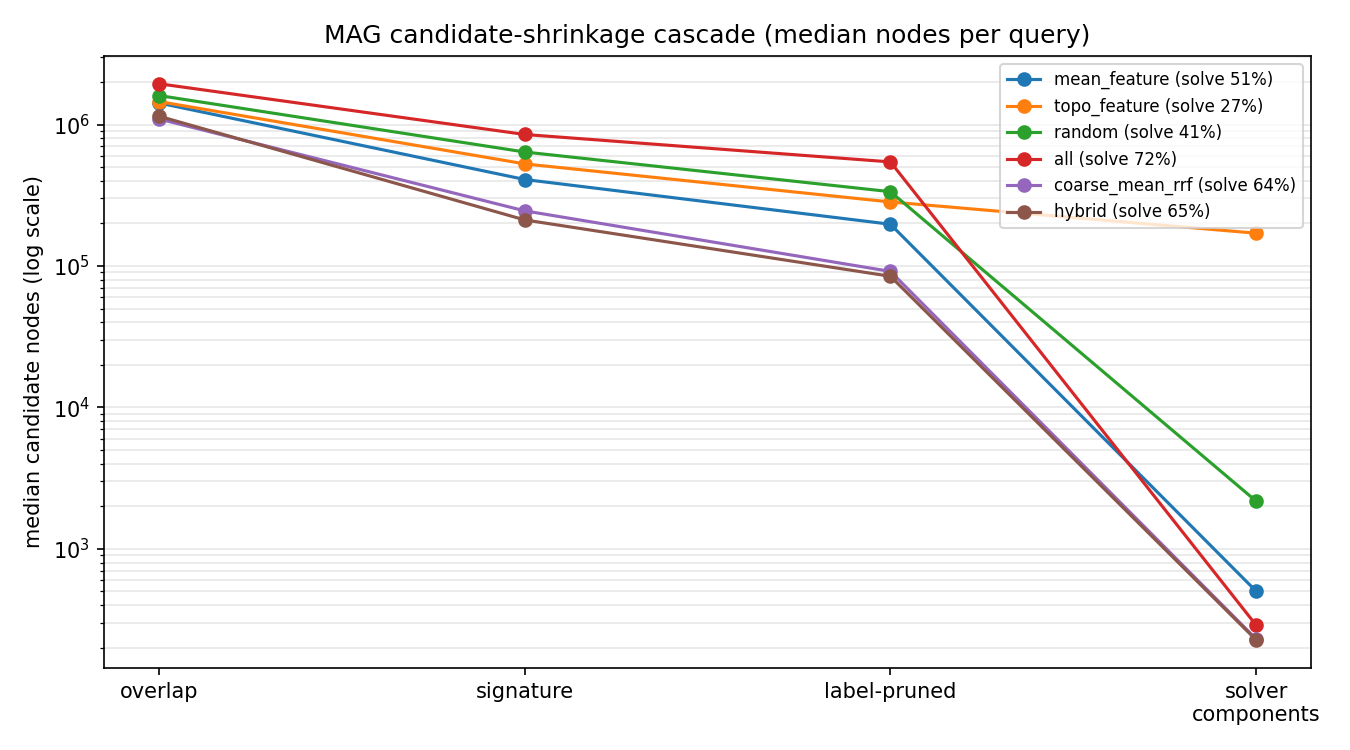
\includegraphics[width=0.86\textwidth]{fig_candidate_shrinkage_mag.png}
\caption{\textbf{MAG candidate-shrinkage cascade (median nodes per query, log scale).} Each policy's candidate is tracked through overlap, signature, label pruning, and component decomposition. Learned retrieval (Jigsaw) and Mean-RRF reach much smaller solver inputs than uninformed policies, and far smaller than FilterAll, even though all share the same lossless pruning.}
\label{fig:shrinkage}
\end{figure}

\end{document}
